% En esta sección se presenta una breve descripción de la solución que se propone, 
% el principal objetivo de esta sección es poder dar el bosquejo de la solución 
% para que pueda ser evaluado. No es necesario detalles, pero sí mencionar sus 
% componentes generales. 
% Si las tecnologías que se van a utilizar ya están establecidas, se deberán 
% incluir aquí. De no estar definidas todas, enumerar las que sí están definidas 
% y explicar qué consideraciones tendrán en cuenta para definir las restantes.

\noindent Como respuesta a las problemáticas presentadas anteriormente nosotros desarrollamos una arquitectura
completamente distribuida, opuesta totalmente al modelo monolítico prevaleciente en la industria de los videojuegos. 
El estado del juego no se encuentra contenido en un único nodo servidor, sino que se distribuye entre varios, cada uno con igual importancia y responsabilidades que el resto. El conjunto del estado en cada uno de estos nodos compone el 
estado del juego en su totalidad.

El aspecto central del videojuego desarrollado es el uso que hace del \textbf{modelo de actores}.
Dicho modelo se basa en el \textbf{actor} como mínima unidad de cómputo y el pasaje de \textbf{mensajes} como única manera
de compartir información entre los actores. Este paradigma, ideado por Carl Hewitt en los años 70, elimina varios de los problemas presentes
en la programación concurrente tradicional que mencionamos anteriormente, como
los \textit{deadlocks} y \textit{race conditions}, al evitar el uso de memoria compartida
como herramienta de comunicación en el sistema. Resulta, además, en una forma natural de representar a las entidades del videojuego, donde podemos plantear una 
relación \textbf{1 a 1} entre entidad y actor. Si establecemos que el estado de cada entidad 
debería ser administrado por ella misma, otra característica intrínseca del modelo de actores,
se desprende entonces que se ajusta perfectamente a lo que queremos desarrollar, dado que el actor es el único que puede modificar
su propio estado.

Existen muchas implementaciones del modelo de actores. Algunas de ellas son estándar del lenguaje de programación,
como en Erlang y Elixir, otras son bibliotecas de terceros que implementan el paradigma sobre lenguajes
agnósticos al mismo, como es el caso de la biblioteca Actix en Rust o Hollywood en Go.
Nosotros decidimos utilizar Akka, un toolkit para construir aplicaciones concurrentes
y distribuidas que implementa el modelo de actores para la Java Virtual Machine.
Si bien Akka en sí está implementado en Scala, es compatible con otros lenguajes
basados en la JVM, como Java y Kotlin. Particularmente nos decantamos por utilizar Scala también
como lenguaje de programación del proyecto, ya que es el lenguaje nativo de Akka y cuenta con la documentación
más completa y actualizada.

Akka nos permite desarrollar un sistema distribuido
donde nuestra aplicación puede ejecutarse en N nodos de manera transparente, donde los distintos actores que residen en cada nodo
pueden comunicarse entre sí sin importar en cuál se encuentren y desconociendo la ubicación del otro actor con el que se comunican.
En breve entraremos en más detalle sobre el funcionamiento de Akka y los distintos componentes que utilizamos.

No alcanza sin embargo únicamente con Akka para poder desarrollar la arquitectura de nuestro videojuego.
El primer punto a resolver con el que nos encontramos es que necesitamos un mecanismo que nos permita comunicar distintos eventos
provenientes de un jugador a los otros jugadores. Una primera solución que se podría plantear a esta problemática sería que cuando un jugador realice una acción,
por ejemplo de movimiento, sea responsabilidad de este notificar vía mensajes a todos los demás jugadores que se ha desplazado. Esta solución sin embargo no es escalable, principalmente por dos motivos:

\begin{itemize}
    \item Cada actor correspondiente a un jugador debería almacenar una referencia a todos los demás jugadores para poder notificarles los eventos.
    Dados N actores en el sistema, esto generaría una complejidad espacial de O($N^2$), además de incurrir una penalidad temporal de O($N$) en el procesamiento de cada evento
    del jugador.
    \item No contamos con un mecanismo que nos permita notificar a los demás actores que un nuevo actor se ha unido al sistema de forma automática.
    Para que un actor conozca a otro depende de haber recibido su dirección a través de un mensaje o haberlo creado él mismo.
\end{itemize}

El segundo punto podría resolverse si utilizamos un actor central el cual es el encargado de crear a todos los actores de los jugadores
y almacenar las referencias a cada jugador creado, pero este mecanismo presenta un único punto de falla en el sistema, algo que queremos evitar a toda costa
para poder maximizar la distribución del modelo desarrollado.

Debido a esto, y siempre con el objetivo de maximizar la distribución del sistema minimizando los puntos de falla únicos del mismo,
decidimos hacer uso de otra tecnología distribuida, \textbf{Kafka}.

Kafka es un sistema distribuido de procesamiento de datos y almacenamiento de eventos caracterizado
por alto \textit{throughput} y baja latencia, características críticas para los sistemas de tiempo real.
Kafka se adapta perfectamente a lo que necesitamos para poder comunicar los eventos que los jugadores
realicen dentro del juego, y nos permite implementar un protocolo de comunicación de eventos entre los actores
de baja latencia, alta disponibilidad, y tolerante a fallos.

Integrando Kafka en el sistema diseñamos un mecanismo de comunicación de eventos donde delegamos la lectura
y publicación de eventos en Kafka a actores específicos, de aquí en adelante denominados \textbf{Consumidores}
y \textbf{Productores}. Los Productores son los encargados de publicar en un tópico de Kafka los eventos de notificación masiva
que un jugador realice en el juego, como por ejemplo un movimiento o un mensaje de chat a la sala, y los Consumidores
son los encargados de leer estos eventos y notificar a los actores correspondientes de los demás jugadores.
Este último paso, la notificación del Consumidor a los demás jugadores de la partida, no es trivial de implementar.
A primera vista, volvemos al problema inicial de que deberíamos almacenar referencias a todos los actores del juego registrados
para poder enviarles los mensajes de notificación. Una forma de evitar esto podría ser proponer que cada jugador tenga un correspondiente
Consumidor, lo que tiene la ventaja de no introducir un punto único de falla. En la práctica los consumidores de Kafka consumen muchos recursos y
nuestro servidor sería incapaz de procesar una gran cantidad de jugadores.
Es aquí donde introducimos otro de los principales \textit{features} de Akka que nos permite resolver esta problemática:
\textbf{Akka Streams}.

Akka Streams es una implementación de Akka de la iniciativa \textit{Reactive Streams}, un estándar para el procesamiento de datos de forma asincrónica y no bloqueante.
En particular, Akka Streams permite definir \textit{pipelines} de procesamiento de datos a los cuales se les pueden aplicar distintas transformaciones y operaciones.
La clave detrás del uso de Akka Streams es que permite conectar múltiples fuentes de datos con múltiples consumidores de forma eficiente y sin bloqueos. Es similar a
lo que ya hacemos con Kafka, pero a nivel del nodo de la aplicación, es decir, internamente, y con la ventaja de necesitar considerablemente menos recursos que con
consumidores de Kafka.

Los eventos masivos, entonces, se procesan de la siguiente manera:

\begin{itemize}
    \item Un jugador realiza una acción en el juego, como por ejemplo  un movimiento.
    \item El actor correspondiente al jugador envía un mensaje al Productor con el evento.
    \item El Productor publica el evento en un tópico de Kafka.
    \item Un Consumidor lee el evento del tópico de Kafka y lo envía por un \textit{stream}.
    \item Cada uno de los demás jugadores del nodo recibe el evento a través del \textit{stream}.
\end{itemize}

\begin{figure}[htbp]
    \centering
    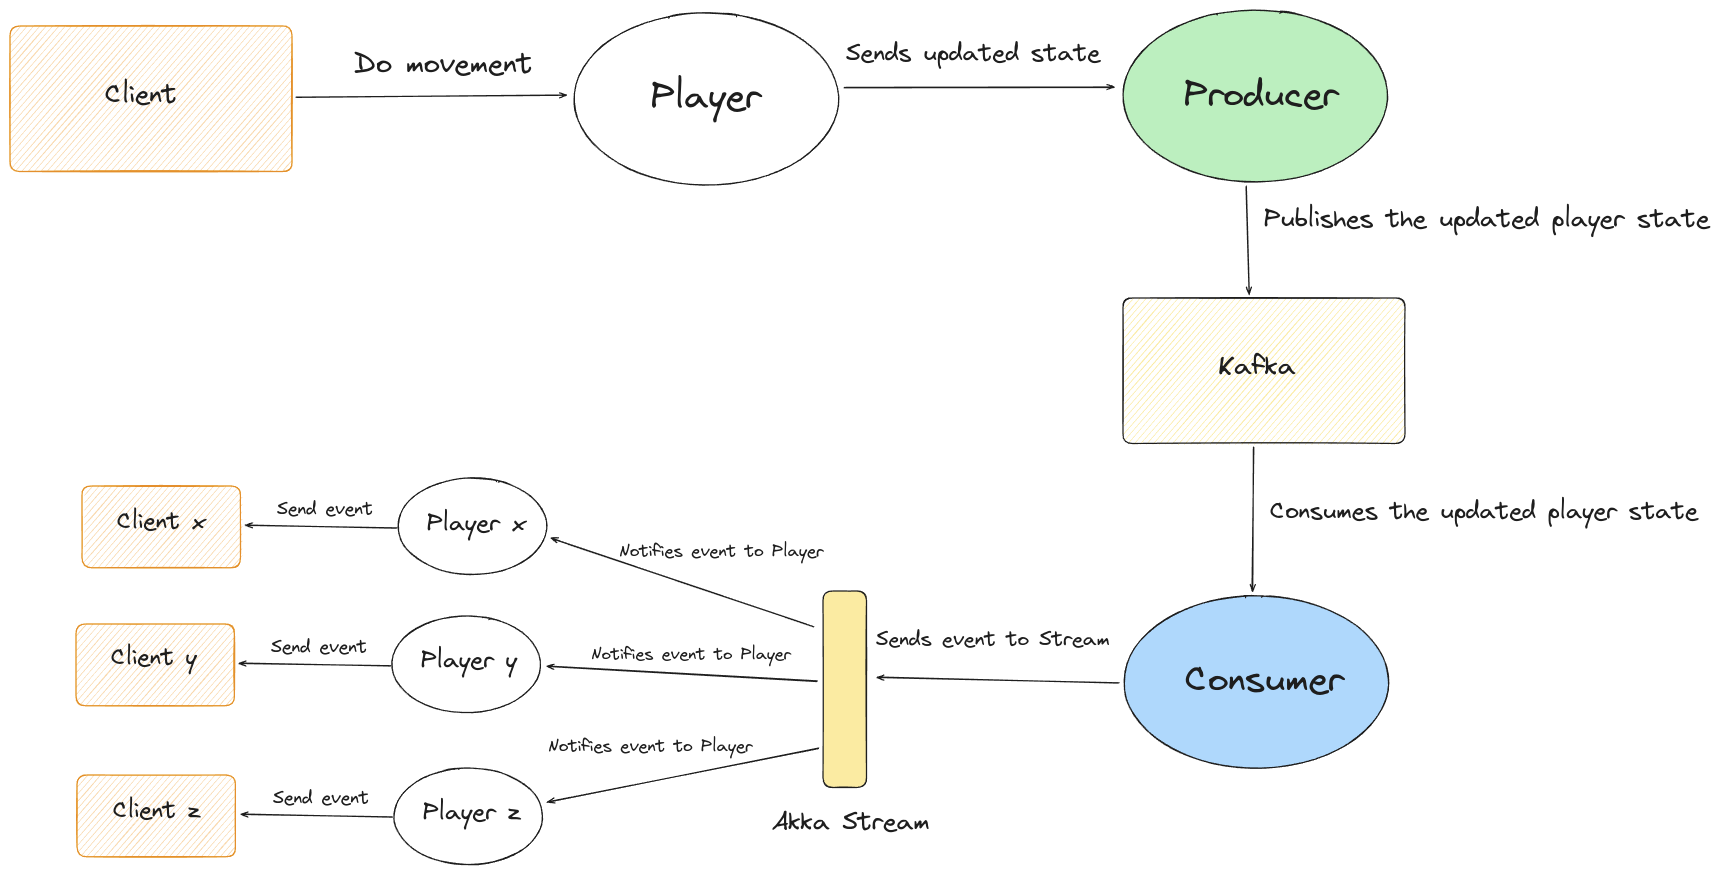
\includegraphics[width=1.0\textwidth]{../assets/introduction-architecture.png}
    \caption{\textit{Overview} simplificado de la arquitectura propuesta.}
\end{figure}

Este diagrama resume la arquitectura desarrollada de forma simplificada. Es importante recordar que lo descrito corresponde a un único nodo del sistema.
La clave de la escalabilidad de la aplicación es que podemos replicarlo en N nodos, donde cada uno de ellos es responsable de un subconjunto de los jugadores,
y la comunicación entre los actores que representan a esos jugadores es transparente a la ubicación del actor en los nodos del sistema, dando la ilusión de que la ejecución está contenida en un único nodo.

\subsection{Introducción a Akka}

\noindent Akka cuenta con varias herramientas para conseguir implementar la arquitectura explicada previamente. Para poder entender los distintos componentes de nuestro servidor
es necesario primero introducir cada tecnología de Akka que utilizamos y dar una breve pero clara explicación de sus usos y funcionalidades.
Comenzamos por lo central: la implementación del modelo de actores en Akka. 

\subsubsection{Akka Actors Typed}

\noindent El corazón de Akka es el modelo de actores. Es su principal componente y sobre el cual se construyen todos los demás.
Históricamente Akka implementaba a los actores como clases de Scala que heredan de una clase \textbf{Actor}.
La clase luego debe implementar un método \textit{receive} que se encarga de definir el comportamiento del actor según el mensaje recibido.
Dicho método recibe el mensaje como argumento del mismo, donde el mensaje puede \textbf{ser cualquier tipo de dato de Scala}.
Mediante Pattern Matching, un feature nativo de Scala, se define el comportamiento del actor según el tipo de mensaje recibido.
El problema con esta implementación es que se pierde todo tipo de validación de tipos en tiempo de compilación.

Como respuesta a esta problemática, Akka introdujo una nueva versión de la biblioteca de actores llamada \textit{Akka Actors Typed}.
Esta nueva versión introduce el concepto de tipado para los mensajes que pueden recibir los actores, y además mantiene compatibilidad
con los actores de la versión anterior, renombrada a \textit{Akka Actors Classic}.

A continuación se muestra una comparación entre la definición de un actor en la versión clásica y su análogo en la versión tipada.

\newpage

\begin{lstlisting}[language=Scala, caption={\textbf{Ejemplo de Actor en Akka Actors Classic}}]
    import akka.actor.{Actor, ActorSystem, Props}

    // Define the messages
    case object Increment
    case object Decrement
    case object Print
    
    // Define the Counter actor
    class Counter extends Actor {
      var count = 0
    
      def receive = {
        case Increment => count += 1
        case Decrement => count -= 1
        case Print     => println(s"Current count is $count")
      }
    }
\end{lstlisting}

\begin{lstlisting}[language=Scala, caption={\textbf{Ejemplo de Actor en Akka Actors Typed}}]
    import akka.actor.typed.scaladsl.Behaviors
    import akka.actor.typed.{ActorSystem, Behavior}
    
    // Define the messages
    sealed trait Command
    case object Increment extends Command
    case object Decrement extends Command
    case object Print extends Command
    
    // Define the Counter actor
    object Counter {
      def apply(): Behavior[Command] = counter(0)
    
      private def counter(count: Int): Behavior[Command] = {
        Behaviors.receiveMessage {
            case Increment =>
                counter(count + 1)
            case Decrement =>
                counter(count - 1)
            case Print =>
                println(s"Current count is $count")
                Behaviors.same // Reuses the current behavior
        }
      }
    }
\end{lstlisting}

Como se puede observar, Akka Classic tiene un enfoque orientado a objetos para los actores.
El estado del actor se mantiene en variables de instancia y el comportamiento del actor se define en la función
\textit{receive} heredada de la clase \textit{Actor}. En cambio, Akka Typed tiene un enfoque funcional, donde el comportamiento
del actor se define mediante la función \textit{Behaviors.receiveMessage}, que es una \textit{factory} de comportamientos.
En Akka Typed un actor se define por su \textit{behavior}, el cual es una función que determina el comportamiento del actor
frente a todos los distintos mensajes que acepta. Luego de procesar cada mensaje debe devolverse el siguiente comportamiento.
El estado del actor se mantiene en los argumentos de la función comportamiento, y no en variables de la instancia.

Nuestro servidor de \textit{Fiubakka} hace uso exclusivo de la nueva API de Akka Typed, pero es importante estar al tanto
de la versión Akka Classic, ya que muchos proyectos existentes todavía la utilizan.

\subsubsection{Akka Cluster}

\noindent Anteriormente mencionamos que existen implementaciones del modelo de actores para distintas tecnologías. Si nos limitásemos
únicamente a utilizar el componente de actores de Akka no habría un motivo diferencial, más allá de la preferencia de lenguaje
o recursos disponibles en la web, para elegirlo sobre otras implementaciones. Akka Cluster es el primer motivo, y el más importante,
de por qué usamos Akka para implementar nuestro videojuego.

Akka Cluster extiende el modelo de actores de \textbf{forma transparente a la aplicación} para poder formar un \textit{cluster} de nodos de Akka,
comunicados entre sí, donde los actores pueden enviarse mensajes entre ellos sin importar el nodo en el que residan. Esto posibilita agregar
más poder de cómputo de forma \textbf{horizontal} al sistema. Siempre y cuando el problema que estemos resolviendo en Akka se beneficie de mayor
concurrencia y paralelismo, podemos agregar más nodos al cluster para distribuir la carga y conseguir mejores resultados en lugar
de tener que mejorar el hardware del sistema que tuviese que ejecutar la aplicación.

Otro problema que Akka permite resolver mayormente de forma transparente es la serialización de los mensajes de los actores. Cuando los actores que se comunican
residen en distintos nodos es necesario serializar los mensajes para poder enviarlos a través de la red, ya sea via TCP o UDP. Por defecto, Akka utiliza conexiones
TCP entre los nodos para la comunicación de los mensajes de los actores, aunque es posible configurar la conexión vía UDP (como es el caso de la configuración de nuestro proyecto).
Independientemente del procotolo de comunicación es necesario serializar los mensajes, y Akka provee una dependencia que nos permite definir a los mensajes como extensiones
de un \textit{trait} o interfaz de Scala, y luego automáticamente se encarga de serializar y deserializarlos en caso de que necesiten viajar por la red.

Inicializar un cluster de Akka es sencillo. A modo de ejemplo, esta es la configuración de \textit{Fiubakka}
para el ambiente local de desarrollo:

\label{config:akka-cluster}
\begin{lstlisting}[language=applicationconf, caption={\textbf{Configuración de Akka Cluster Fiubakka}}]
    cluster {
        downing-provider-class = "akka.cluster.sbr.SplitBrainResolverProvider"
        shutdown-after-unsuccessful-join-seed-nodes = 60s
        seed-nodes = ["akka://fiubakka-server@127.0.0.1:2020"]

        sharding {
            number-of-shards = 100
            least-shard-allocation-strategy.rebalance-absolute-limit = 20
            buffer-size = 300000
            updating-state-timeout = 15 s
        }
    }
\end{lstlisting}

Para el ambiente local se utilizan lo que se denomina como \textit{seed nodes} o nodos semilla, que son nodos que se encargan de iniciar el cluster.
Al iniciar un nodo de Akka el mismo verifica si su dirección corresponde a un nodo semilla. Si es así, se encargará de escuchar futuras
conexiones de otros nodos que busquen unirse al cluster, y siempre que un nodo no semilla se inicie intentará conectarse a los nodos semilla especificados
en la configuración. Por supuesto, este método únicamente funciona si las direcciones de los nodos son estáticas y conocidas de antemano.
Para ambientes dinámicos, como por ejemplo Kubernetes, existen otros métodos de descubrimiento de nodos que describiremos más adelante.

La sección de \textit{sharding} incluida en la configuración nos lleva a nuestro siguiente componente de Akka del que \textit{Fiubakka}
hace uso: \textbf{Akka Cluster Sharding}, una extensión de las funcionalidades que Akka Cluster provee.

\subsubsection{Akka Cluster Sharding}

\noindent Una problemática que surge al utilizar Akka Cluster es que si bien los actores pueden comunicarse entre sí sin importar en qué nodo
se encuentren, es necesario de alguna forma conseguir la referencia a los actores que residen en nodos ajenos al propio. En principio
pueden utilizarse llamados remotos a los demás nodos y conseguir como respuesta las direcciones de los actores que nos interesan para poder
crear la referencia a los mismos, pero no es ideal. Por otro lado, una propiedad deseable en los sistemas distribuidos es la capacidad
de esparcir la carga entre los distintos nodos \textbf{elásticamente}, esto es, que el incremento y decremento de nodos en el cluster
resulte en un balanceo uniforme de la carga total.

Akka Cluster Sharding es, entre otras cosas, una respuesta a ambos puntos. Permite crear \textbf{entidades} que pueden ejecutarse en cualquier nodo
del cluster y que pueden ser referenciadas desde cualquier nodo por medio de un identificador único, para poder comunicarnos con las mismas.
Podemos pensar a una entidad como un actor que reside en un único nodo del cluster para todo determinado momento, y al cual podemos conseguir una referencia sin saber
en qué nodo se encuentra, utilizando su identificador.

Además, Sharding nos permite definir una \textbf{estrategia de balanceo} de las entidades al momento de creación de las mismas,
y de \textbf{rebalanceo} al modificarse la composición de los nodos del cluster. Nuevamente, para nuestra aplicación, estos balanceos son
completamente transparentes. Si un nodo se cae, las entidades que residían en el mismo son automáticamente reubicadas en otros nodos del cluster,
y los distintos actores que estuviesen comunicándose con dichas entidades no se enterarán del cambio.

Sin adentrarnos demasiado en los detalles, Cluster Sharding consigue implementar esto de la siguiente forma.
En primer lugar, por cada tipo de entidad existirá lo que se conoce como un \textit{Shard Coordinator}, un actor singleton
que residirá en el nodo líder del Akka Cluster y será el responsable de determinar en que nodos del cluster residirá
un \textit{shard}. Los shards son conjuntos de entidades, donde cada entidad tiene un shard asignado mediante un hash calculado sobre su
identificador único. En este sentido, la mínima unidad asignable por el Shard Coordinator es el shard, y no entidades individuales (de allí su nombre).
Cada nodo tendrá lo que se denomina un \textit{Shard Region} por cada tipo de entidad, un actor que se encargará de administrar los shards del nodo
que le hayan sido asignados por el Coordinator, así como resolver, también mediante el Shard Coordinator en caso de ser necesario, las ubicaciones
de los shards cuyas entidades sean comunicadas por los actores del nodo.

En el caso de nuestra aplicación \textit{Fiubakka}, cada cliente que se conecta al juego va a generar dos entidades asociadas: una entidad
\textbf{Player} y otra entidad \textbf{PlayerPersistor}. La ventaja de representar a los jugadores como entidades en lugar de actores es justamente que conseguimos
referenciar a un jugador sin conocer ni importar el nodo en el que reside, y que además son sujetos a los procesos de balanceo de carga que se hacen sobre las entidades.
Esto nos permite escalar horizontalmente frente al incremento de jugadores en el juego, mediante el agregado de nodos de forma dinámica.

Las entidades definidas tienen una diferencia muy marcada con los actores y es que son automáticamente iniciadas siempre que reciban un mensaje. Dado que pueden ser referenciadas
desde cualquier actor (u otra entidad) en el cluster, el actor que envía el mensaje desconoce si la entidad está funcionando o no. Debido a esto, Akka Cluster Sharding implementa como mecanismo
la inicialización automática de las entidades al recibir un mensaje, cualquiera sea el tipo u origen del mismo. Este mecanismo, sin embargo, introduce una problemática. Si las entidades pueden iniciarse
en cualquier momento, tendríamos que implementar algún proceso que se encargue periódicamente de detener a las entidades cuando no se estén utilizando para liberar los recursos.

Afortunadamente Cluster Sharding tiene esto en cuenta y lo soluciona mediante un mecanismo automático de \textbf{pasivación} cada cierta cantidad de tiempo (valor configurable, por defecto
son 2 minutos). La pasivación se trata de detener a todas aquellas entidades que no hayan recibido ningún mensaje en el tiempo de \textit{timeout} definido. Esto garantiza que no se malgastan recursos
en entidades poco utilizadas y quita responsabilidad al programador de tener que estar administrándolas manualmente. Por supuesto, una entidad pasivada será reiniciada al momento en el que vuelva a recibir un mensaje.

\begin{figure}[htbp]
    \centering
    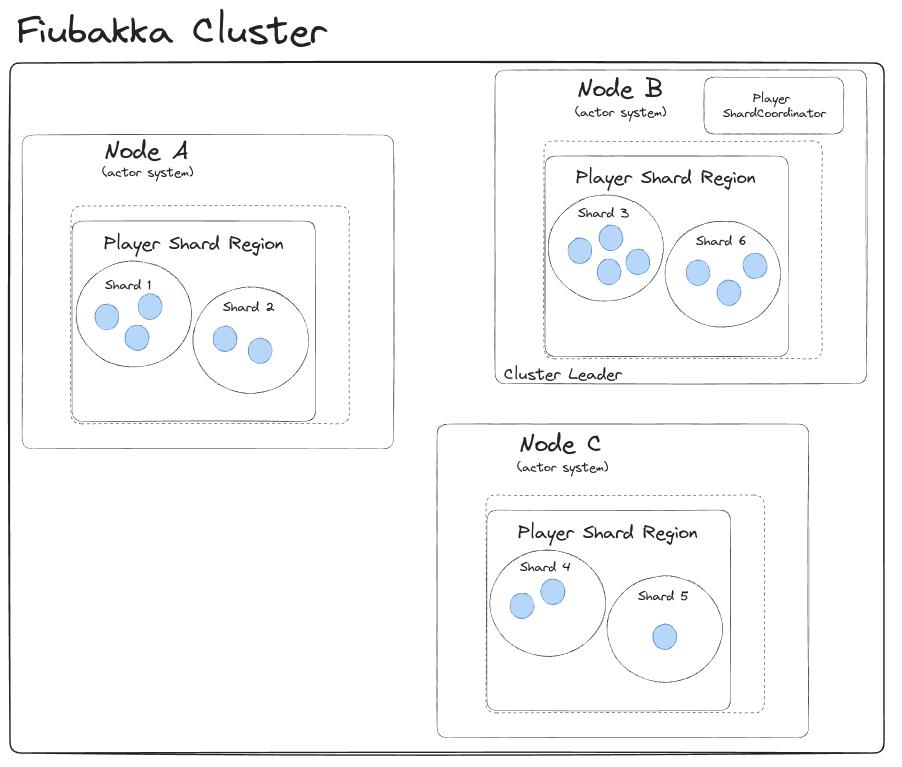
\includegraphics[width=0.6\textwidth]{../assets/cluster-sharding-example.jpeg}
    \caption{Ejemplo de Cluster Sharding para la entidad Player}
\end{figure}

\newpage

Es claro entonces la importancia que tiene Cluster Sharding en nuestro modelo, y tiene un papel fundamental, junto con Akka Cluster, en permitirnos desarrollar nuestra arquitectura
propuesta. Implementaciones del modelo de actores como \textit{Actix} no cuentan con ningún feature similar. Por otro lado, Elixir sí que cuenta con capacidades similares a las de Akka
Cluster, aunque no las de Cluster Sharding ni las del siguiente componente clave: Akka Persistence.

\subsubsection{Akka Persistence}

\noindent Cluster Sharding nos da la garantía de que las entidades se reinician en caso de error o eliminación de un nodo del cluster, además de rebalancearlas al agregarse un nuevo
nodo. En principio, únicamente con los componentes de Akka que presentamos hasta ahora, ambos casos resultan en un problema: si la entidad se vuelve a iniciar, estaríamos perdiendo el estado
de la misma, ya que el estado de los actores está en memoria. Esto resultaría por ejemplo en perder los datos de posición del jugador, su equipamiento y cualquier otra información asociada.
En arquitecturas \textit{stateless}, el estado sería persistido en una base de datos externa ante cada cambio sucedido.
Una propuesta más que válida sería persistir el estado del actor serializado como si se tratase de un objeto. Akka Persistence toma esta idea y la integra nativamente en los actores. 

Existen dos \textit{flavors} o implementaciones de Akka Persistence. La primera es Event Sourcing, la cual se basa en un proceso de replay de eventos. Cada evento sucedido genera en respuesta
un comando que es procesado por el actor, y el procesamiento de todos los comandos provenientes de los eventos determina el estado final del actor. Lo que se persisten en ese caso son justamente los eventos.
En caso de que el actor se reinicie, se leen los eventos persistidos y se reenvían los comandos correspondientes al actor para volver al estado en el que se encontraba previo a su caída.
Lógicamente, dado que en el tiempo pueden acumularse muchos eventos, se introduce un concepto de \textit{snapshot} del estado del actor que actúa como un checkpoint. Cada N cantidad de eventos
se almacena el snapshot y se reinician los eventos persistidos, tomando ese snapshot como estado inicial previo al reprocesamiento de los eventos. Esto evita que las inicializaciones
del actor sean muy costosas en tiempo.

Esta primera versión resulta útil en sistemas donde llevar un registro de los sucesos resulte valioso. En el caso de \textit{Fiubakka} no nos interesa entender los eventos
que llevaron al estado actual de un jugador, únicamente necesitamos el estado cada ciertos instantes o acciones.
Afortunadamente, Akka Persistence introdujo en una de sus últimas versiones otra alternativa llamada \textbf{Durable State}.

Durable State permite definir \textit{behaviors} que se caracterizan por generar lo que se denomina un \textit{effect} por cada comando recibido en el actor.
En la nomenclatura funcional, la cual vimos anteriormente que Akka Typed utiliza, un efecto hace referencia a una acción secundaria al resultado de la función.
Dado que en Akka Typed todo mensaje que un actor procesa tiene como resultado de la función el nuevo comportamiento, los efectos incluyen acciones como persistir el estado del actor
en la base de datos o responder al actor que envió el mensaje.

Este modelo de persistencia de actores se ajusta casi perfectamente a lo que buscamos para persistir el estado de los actores de los jugadores.
El único problema, en la práctica, es que la API de Durable State Behavior es algo limitada. No es posible por ejemplo tener como efecto tanto la persistencia del actor
como la respuesta al actor que envió el mensaje. Además, en el caso de generar como efecto la persistencia del estado del actor, el mismo no procesará el siguiente mensaje hasta no haberse
ejecutado el almacenamiento en la base de datos. Dado que la ejecución de las consultas a la base de datos puede llevar un tiempo no despreciable comparado con la velocidad de los actores en el procesamiento de los mensajes,
preferimos no utilizar Durable State Behavior directamente sobre las entidades \textbf{Player} asociados a cada cliente del juego.
En cambio, definimos otra entidad \textbf{PlayerPersistor} que sí utiliza Durable State Behavior y al cual el Player le envía su estado en un mensaje.
De esta forma desacoplamos la persistencia del estado del jugador del procesamiento de los eventos que reciba, evitando incrementar la latencia y empeorar la experiencia del juego.

Dado que un jugador puede recibir miles de mensajes por segundo de distintos eventos que van sucediendo en el juego, optamos por enviar el mensaje de persistencia al
PlayerPersistor cada cierta cantidad de segundos para alivianar la carga en la base de datos. En la práctica perdernos unos segundos de movimiento del jugador es irrelevante, ya que ante eventos
importantes (por ejemplo cuando el jugador se desconecta) persistimos el estado inmediatamente, por lo que en general el jugador verá su estado de forma correcta
al reconectarse al juego.

A continuación se muestra la implementación del \textbf{PlayerPersistor}, el actor responsable de persistir el estado del jugador en el servidor.

\begin{lstlisting}[language=Scala, caption={\textbf{Implementación del PlayerPersistor}}]
object PlayerPersistor {
    sealed trait Command extends CborSerializable
    final case class Persist(newState: DurablePlayerState) extends Command
    final case class GetState(replyTo: ActorRef[GetStateResponse]) extends Command
    
    final case class GetStateResponse(state: DurablePlayerState)
        extends CborSerializable
    
    val TypeKey = EntityTypeKey[Command]("PlayerPersistor")
    
    def apply(persistenceId: PersistenceId): Behavior[Command] = {
        DurableStateBehavior[Command, DurablePlayerState](
            persistenceId,
            emptyState = DurablePlayerState(
                "",
                Position(845, 1730),
                Equipment(0, 0, 0, 0, 0, 0, 0),
                0
            ),
            commandHandler = commandHandler
        )
    }
    
    private def commandHandler(
        state: DurablePlayerState,
        command: Command
    ): Effect[DurablePlayerState] = {
        command match {
            case Persist(newState) => {
                Effect.persist(newState)
            }
            case GetState(replyTo) => {
                replyTo ! GetStateResponse(state)
                Effect.none
            }
        }
    }
}
\end{lstlisting}

Nótese como el PlayerPersistor combina el concepto de entidad de Akka Cluster Sharding con el de persistencia de Akka Persistence. En la práctica, ambos están muy relacionados,
ya que las entidades suelen tener un estado asociado que necesita ser recuperable.

Como base de datos para la persistencia tanto del estado de los actores como de otros registros de información utilizamos
\textbf{PostgreSQL}. Otras opciones que Akka Persistence soporta nativamente son Cassandra y MongoDB.

\subsubsection{Akka Streams}

\noindent El último componente principal de Akka que utilizamos es uno que mencionamos en el resumen de la arquitectura: Akka Streams.
Se trata de una implementación de la iniciativa de Reactive Streams, un estándar para el procesamiento de datos de forma asincrónica y no bloqueante.
Conceptualmente, consiste en un \textit{pipeline} de procesamiento de datos, donde tenemos tres componentes principales: el \textbf{Source},
el \textbf{Flow} y el \textbf{Sink}. El Source es la fuente de los datos, el Flow es una etapa interna del pipeline que transforma los datos, y el
Sink es el consumidor final. Todo Stream tiene al menos un Source y un Sink, y puede tener cualquier cantidad (o ningún) Flow entremedio.

Un Stream es un maquetado o \textit{blueprint} de cómo los datos van a ser procesados. La acción de construir el Stream y ejecutarlo se denomina
\textit{materializar} el Stream. El Stream puede ser materializado una única vez, ya que la fuente de datos (Source) puede ser consumida una única vez.

Se trata de una herramienta particularmente útil para procesar grandes cantidades de datos de forma eficiente. Cada etapa del Stream puede ser procesada
concurrentemente en distintos hilos del procesador, lo que garantiza un alto \textit{throughput}. Es posible construir pipelines extremadamente complejos de forma relativamente
sencilla, y cuenta con muchos operadores nativos que facilitan la construcción de los mismos. No apunta a la simplicidad de uso, sino a proveer todos los elementos
básicos necesarios sobre los cuales puede construirse prácticamente cualquier solución.

\begin{figure}[htbp]
    \centering
    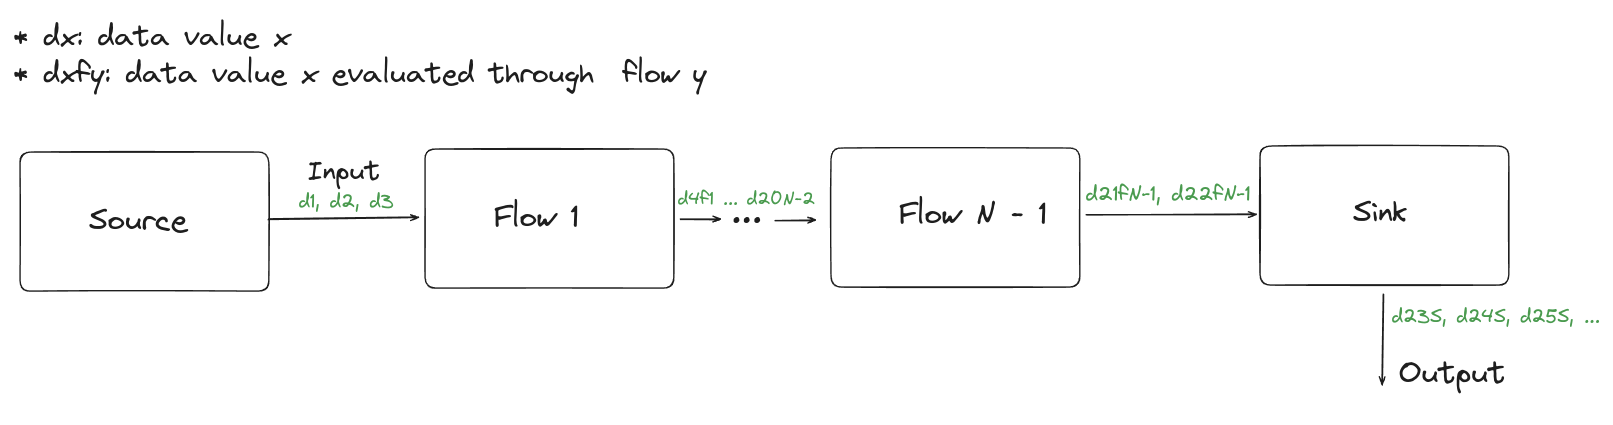
\includegraphics[width=1.0\textwidth]{../assets/akka-stream-example.png}
    \caption{Ejemplo de un Stream lineal con N Flows, un Source y un Sink}
\end{figure}

Akka Streams cuenta nativamente con implementaciones para distintos tipos de fuentes de datos, por ejemplo para el manejo de conexiones UDP o TCP.
Las conexiones de nuestro servidor con los clientes son manejadas mediante Akka Streams en lugar de usar explícitamente las primitivas de sockets,
como uno típicamente haría en un servidor convencional. No solo eso, sino que siempre y cuando uno tenga definido un Source o un Sink
para \textbf{cualquier} fuente de datos, automáticamente pasamos a poder procesar los datos de una única forma agnóstica al protocolo que produce o consume
los datos. Si bien es posible definir uno mismo su propio Source o Sink en caso de necesitarlo, existen implementaciones de casi cualquier tipo que uno puede
pensar. Una implementación ya existente para Kafka se provee dentro de la biblioteca de \textbf{Alpakka}, que agrupa conectores de Akka Streams (Source y Sink)
para una gran variedad de tecnologías. Lógicamente, para la comunicación de eventos del juego entre los actores vía Kafka que explicamos al comienzo, hacemos
uso también de Akka Streams. Los conectores provistos por Alpakka para Kafka encapsulan las primitivas de Consumidor y Productor que Kafka define,
por lo que desde la perspectiva de nuestra aplicación simplemente definimos un Source y un Sink como corresponda y nos abstraemos de los detalles de implementación.

\begin{lstlisting}[language=Scala, caption={\textbf{Ejemplo de un Akka Stream}}]
// A source of integers from 1 to 10.
val source = Source(1 to 10)

// A flow that multiplies each element by 2.
val flow = Flow[Int].map(_ * 2)

// A sink that prints each element.
val sink = Sink.foreach[Int](println)

val runnableGraph = source.via(flow).to(sink)

// Run the graph. Here we are materializing the Stream.
runnableGraph.run()
\end{lstlisting}

\subsection{Arquitectura de Fiubakka}

\noindent Con todos los módulos de Akka presentados, podemos ahora proceder al detalle de nuestra implementación y los distintos componentes
que la conforman. Haremos una descripción partiendo desde la capa de comunicación hasta la de infraestructura de nuestra aplicación, para enteder el flujo completo del procesamiento de
los jugadores en el juego.

\subsubsection{Conexión de los clientes}
\label{sec:client-connection}

\noindent Comenzamos entonces por el punto de entrada de conexión del cliente. El servidor está configurado para exponer un \textit{listener} de TCP en el puerto 2020.
Este listener es manejado por el actor \textbf{PlayerAcceptor} mediante la creación de un Akka Stream que recibe como elementos
conexiones TCP entrantes que corresponden a los clientes del juego. En el caso de que haya múltiples nodos de la aplicación ejecutados (es decir, un Akka Cluster
formado) tendremos un actor PlayerAcceptor en cada nodo del juego, y los clientes podrían conectarse a cualquiera de los nodos para comenzar a jugar.

\begin{lstlisting}[language=Scala, caption={\textbf{Actor PlayerAcceptor}}]
object PlayerAcceptor {
    sealed trait Command
    final case class Accept(connection: Tcp.IncomingConnection) extends Command

    def apply(): Behavior[Command] = {
        Behaviors.setup(ctx => {
            implicit val mat = Materializer(ctx)

            val connections
                : Source[Tcp.IncomingConnection, Future[Tcp.ServerBinding]] =
                Tcp(ctx.system).bind(
                "0.0.0.0",
                ctx.system.settings.config.getInt("game.player-acceptor.port")
                )
            connections.runForeach { connection =>
                ctx.self ! Accept(connection)
            }

            Behaviors.receiveMessage {
                case Accept(connection: Tcp.IncomingConnection) => {
                    ctx.spawn(
                        PlayerHandler(connection),
                        s"PlayerHandler-${connection.remoteAddress
                            .getAddress()
                            .getHostAddress()}-${connection.remoteAddress.getPort()}"
                    )
                    Behaviors.same
                }
            }
        })
    }
}
\end{lstlisting}

Cada conexión recibida en el servidor se procesa a través del mensaje \textbf{PlayerAcceptor.Accept}.
Se crea un nuevo actor \textbf{PlayerHandler} que será el encargado de administrar la conexión con el cliente, incluyendo
el procesado de los mensajes que reciba y la notificación al cliente de los eventos que sucedan en el juego.

\begin{figure}[htbp]
    \centering
    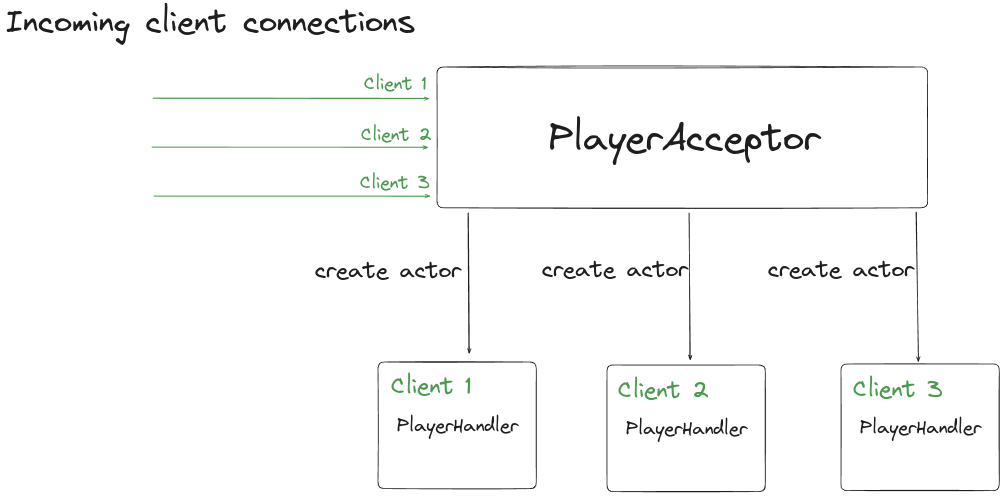
\includegraphics[width=0.8\textwidth]{../assets/player-acceptor.png}
    \caption{Flujo del actor PlayerAcceptor}
\end{figure}

\newpage

El protocolo de comunicación entre el cliente y el servidor será explicado más adelante, en este punto alcanza con entender
que el PlayerHandler realiza la traducción de los datos serializados enviados por el cliente a mensajes internos del actor para su posterior
procesamiento. Dado que la conexión con el cliente está abstraída en un Akka Stream, introducimos un Flow entremedio que tiene como entrada
los \textit{bytes} recibidos y como salida los mensajes internos del actor PlayerHandler. El Sink del Stream es el actor mismo,
por lo que los mensajes serán enviados al PlayerHandler para su procesamiento.

\begin{lstlisting}[language=Scala, caption={\textbf{Stream de conexión del cliente}}]
private def clientStreamHandler(
    ctx: ActorContext[CommandOrPlayerReply],
    conSource: Source[GeneratedMessage, NotUsed]
) = {
    Flow[ByteString]
    .via(
        InMessageFlow(PBClientMetadata, ProtocolMessageMap.clientMessageMap)
    )
    .throttle(60, 1.second) // 60hz tick rate
    .map(commandFromClientMessage)
    .via(
        Flow.fromSinkAndSourceCoupled(
            ActorSink.actorRef(
                ref = ctx.self,
                onCompleteMessage = ConnectionClosed(),
                onFailureMessage = (_) => ConnectionClosed()
            ),
            conSource.via(
                OutMessageFlow(
                (length: Int, `type`: GeneratedEnum) =>
                    PBServerMetadata(
                    length,
                    `type`.asInstanceOf[PBServerMessageType]
                    ),
                ProtocolMessageMap.serverMessageMap
                )
            )
        )
    )
    .instrumentedPartial(
        name = "PlayerHandlerConnection",
        traceable = true,
        reportByName = true
    )
}
\end{lstlisting}

En particular, la función \textbf{commandFromClientMessage} es la que se encarga de traducir los bytes recibidos
en mensajes que el PlayerHandler puede recibir. Los mensajes son enviados mediante el \textit{ActorSink.actorRef}, donde
\textit{ctx.self} es la dirección del actor PlayerHandler.

\begin{figure}[htbp]
    \centering
    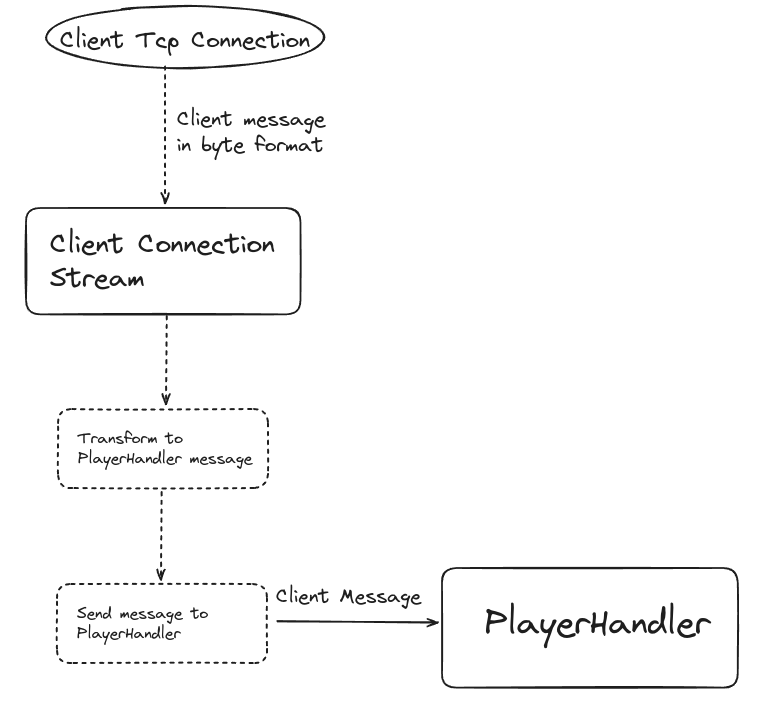
\includegraphics[width=0.7\textwidth]{../assets/player-handler-client-flow.png}
    \caption{Flujo de mensajes del cliente al PlayerHandler}
\end{figure}

\newpage

\subsubsection{Manejo del jugador}

\noindent Hasta aquí explicamos como se conecta un cliente al servidor y como se reciben los mensajes que el cliente emite.
Ahora vamos a explicar como se maneja el estado del jugador y como se integra con todos los demás jugadores que pueden estar
presentes en el juego.

Es necesario aclarar que \textit{Fiubakka} es un \textbf{juego descentralizado} para poder comprender este punto de su estructura. Lo que esto significa es que no existe una
entidad central que maneje el estado de todos los jugadores o que sea origen único del estado del juego en cualquier momento.
Si bien en principio la descentralización puede parecer un problema, es en realidad la principal ventaja (y diferencia) que nuestra arquitectura tiene
frente al modelo monolítico que implementan la mayoría de los videojuegos en línea.

Con el objetivo de disminuir la latencia, evitar bloqueos y dar una mejor experiencia al jugador, todas las acciones que el cliente
realiza \textbf{no requieren de la aprobación del servidor}. En su lugar, el servidor actúa como un replicador y notificador de la información
que el cliente le envía. Si, por ejemplo, el jugador se desplaza, eso genera un mensaje hacia el servidor con el desplazamiento realizado y será luego
responsabilidad del servidor tanto persistir la nueva posición recibida como así también notificar a los demás jugadores del desplazamiento propio.
Ese aviso es parte de los eventos del juego que mencionamos que se realizan a través de Kafka.

De esta forma, lo más cercano a la fuente de la verdad del estado del juego resulta ser la agregación de los estados individuales
de cada jugador almacenados en los clientes conectados al servidor. Si diseñamos el protocolo de mensajes del videojuego de forma tal
que no dependa del orden de llegada de los mensajes ni de la garantía de que todos los mensajes se envíen, podemos valernos de que
el estado de un jugador reportado por el cliente tendrá \textbf{consistencia eventual} en el resto de los jugadores.
Este diseño es clave para la escalabilidad horizontal de la aplicación y la alta performance. Además, implementamos mensajes frecuentes
para cada jugador que reportan el estado del mismo a los demás jugadores, para minimizar el tiempo de posibles inconsistencias en caso de que
sucedieran.

Con todo esto en cuenta es que implementamos la entidad \textbf{Player}. Recordemos de Cluster Sharding que una entidad es un actor que puede residir
en cualquier nodo del cluster y que es susceptible a los procesos de balanceos de carga. La idea de que el Player sea una entidad y no un actor
es que siendo uno de los componentes que más carga de cómputo va a tener en el sistema (tanto de tener que procesar los mensajes del cliente como de otros jugadores)
es necesario que pueda ser reubicado en otros nodos en caso de que la carga sobre el nodo en el que esté residiendo sea elevada.
Además nos garantiza que al conectarse un nuevo cliente al juego se le asigne el Player en el nodo con menor cantidad de \textit{shards} asignados. En la práctica esto
suele coincidir con el nodo con menor consumo de recursos.

La entidad Player maneja el estado del jugador, incluyendo información como su posición o equipamiento. Recordemos que estos datos no son más que una réplica de lo que
el cliente le informa, por lo que el estado del Player y del jugador en el cliente podría no ser exactamente el mismo, aunque eventualmente lo serán debido a la consistencia eventual
que mencionamos anteriormente. Todas las acciones que el cliente realiza o los eventos que van sucediendo en el juego (como pueden ser acciones de otros
jugadores) serán recibidos y procesados por el Player. En el caso de los eventos externos, el Player se encarga de enviar un mensaje
al PlayerHandler notificándole del suceso, para que finalmente el PlayerHandler envíe la información al cliente via la conexión TCP que administra.

El siguiente diagrama muestra conceptualmente el flujo de ejecución del movimiento de un jugador. Es importante aclarar que los diagramas de flujo no logran capturar
el asincronismo del modelo de actores, por lo que el diagrama modela un flujo secuencial. En la realidad el proceso es totalmente asíncrono, ninguno de los actores esperan
la respuesta o completitud de procesamiento de los mensajes enviados.

\begin{figure}[htbp]
    \centering
    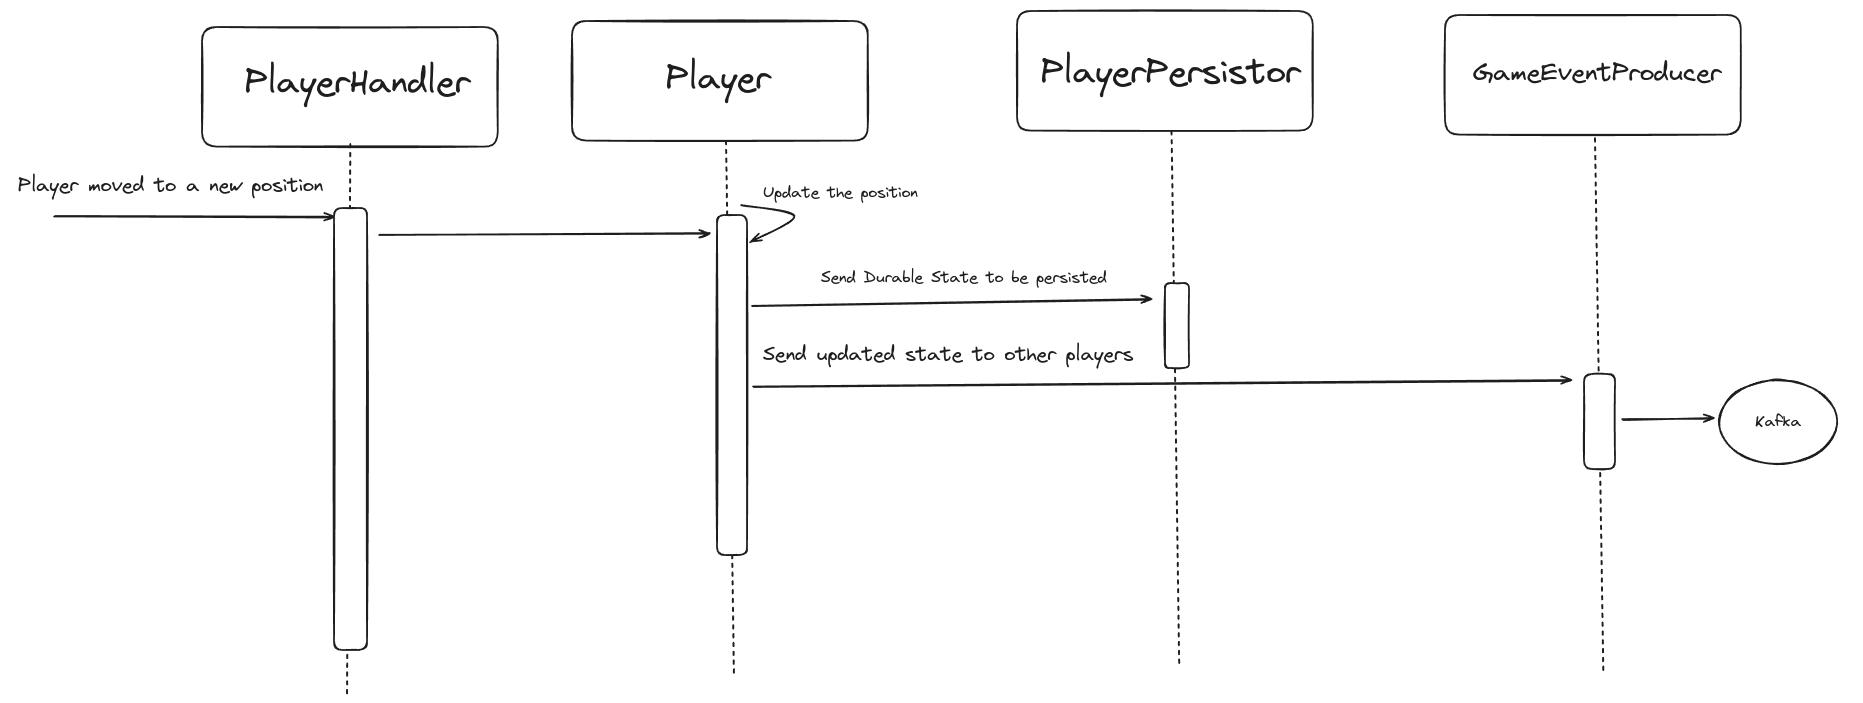
\includegraphics[width=1\textwidth]{../assets/player-movement-example.png}
    \caption{Diagrama de flujo de movimiento de un jugador.}
\end{figure}

\newpage

En el diagrama se muestra un componente que mencionamos previamente cuando presentamos el módulo de Akka Persistence: el PlayerPersistor. Se trata de la entidad encargada de almacenar y recuperar el estado
del jugador. Hace uso de los \textit{behaviors} de Durable State que Akka Persistence provee. Como comentamos anteriormente, la interacción con la persistencia se delega a esta otra entidad y no propiamente al
Player por temas de flexibilidad de API y de latencia. Esto por supuesto significa que no existe garantía de que el nuevo estado haya sido persistido, pero al ser el PlayerPersistor una entidad esta sujeto a las garantías
de Sharding de rebalanceo y recuperabilidad en casos de fallos. En los casos donde haya errores en la persistencia momentáneos podrá recuperarse automáticamente, y dado que el protocolo del juego se basa en mensajes
que garantizan la consistencia eventual del estado del jugador, esta segregación del estado no resulta en fallos críticos. En caso de ser necesario garantizar que una acción se haya persistido,
existen mecanismos dentro de Akka para cerciorarnos de ello.

\subsubsection{Comunicación de los eventos del juego}
\label{sec:events-communication}

\noindent Mencionamos en la introducción a la arquitectura de \textit{Fiubakka} que los eventos que deban ser notificados a todos los demás jugadores se realizan mediante mensajes de Kafka.
La responsabilidad de publicar y consumir estos eventos no recae en sí sobre el Player, sino sobre dos actores que el Player crea al iniciarse: el \textbf{GameEventConsumer} y el \textbf{GameEventProducer}.
Todo Player cuenta con un GameEventProducer para poder notificar sus acciones a los demás jugadores, y con un GameEventConsumer para poder enterarse de las acciones que otros jugadores han realizado.
Lo que en su momento simplificamos como Consumidor y Productor, son en realidad propiamente dicho los consumidores y productores de Kafka, los cuales son el \textbf{Source} y \textbf{Sink} de los \textit{streams}
administrados por el GameEventConsumer y el GameEventProducer, respectivamente.

Cada vez que el Player deba notificar una acción enviará el mensaje con la acción al GameEventProducer. Este se encargará, mediante un Akka Stream conectado a Kafka, de publicar el mensaje
en el tópico correspondiente. Cada mapa del juego tiene su propio tópico de Kafka, por lo que el mensaje se publicará únicamente en el tópico que corresponda al mapa en el que se encuentre el jugador que realizó la acción.
De forma análoga, el GameEventConsumer cuenta con un Akka Stream que tiene como fuente un consumidor del tópico de Kafka correspondiente al mapa en el que el jugador se encuentra. A medida que recibe a través del Stream los
eventos que fueron siendo publicados en el tópico por los demás jugadores, el GameEventConsumer enviará los eventos como mensajes al Player. Por último, el Player se los notificará al PlayerHandler, quien terminará enviándolos
al cliente asignado.

Una consecuencia de este diseño es que los jugadores desconocen en un principio la existencia de los demás. Es únicamente mediante los eventos que van siendo recibidos en el Player provenientes del GameEventConsumer
que el cliente se entera de la existencia de los demás jugadores. Cada acción que un jugador realiza que genera un cambio en su estado dispara el evento de notificación que contiene este nuevo estado actualizado. En el momento que los clientes de los demás jugadores reciben
el evento van a tener visibilidad de la existencia del jugador que envió el evento. Este mecanismo nos permite delegar la agregación del estado de los jugadores al cliente, disminuyendo sustancialmente el uso de los recuros de memoria del servidor.
Cada Player almacenará únicamente su propio estado mientras que el estado de los demás jugadores se le reportará al cliente a medida que se reciban los eventos, pero no se almacena ninguna información de los demás jugadores en la entidad Player.
Por supuesto, además de las actualizaciones, se notifica el estado del jugador cada unos pocos segundos de forma constante para evitar que un jugador que nunca realiza una acción sea invisible al resto.

\begin{figure}[htpb]
    \centering
    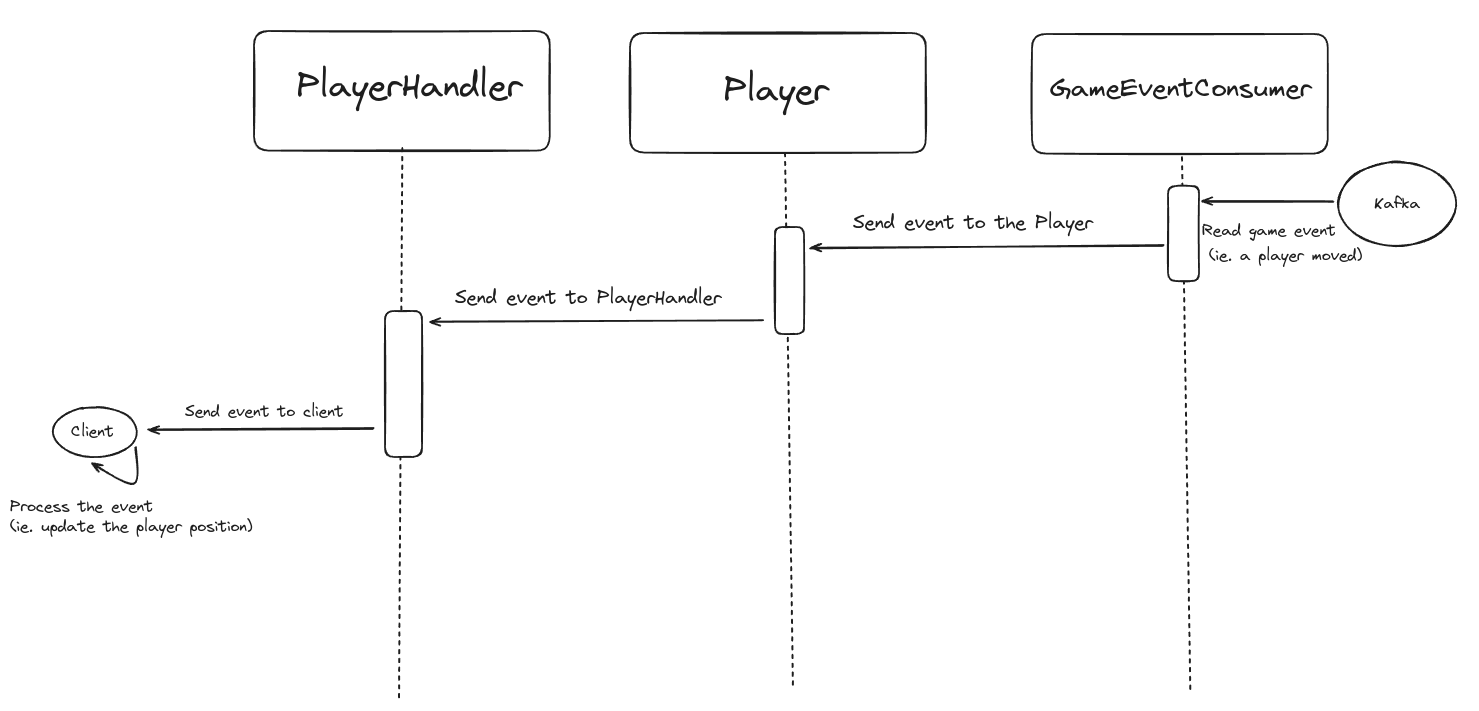
\includegraphics[width=0.8\textwidth]{../assets/game-event-consumer-example.png}
    \caption{Diagrama de flujo de eventos del juego para un Player.}
\end{figure}

Al igual que antes, el diagrama de flujo no captura el asincronismo del modelo de actores. Por otro lado, se observa lo que explicamos respecto a que el estado de los demás jugadores no es persisitido de ninguna forma en el PlayerPersistor,
sino que se delega su manejo al cliente. Es responsabilidad de este mantener el estado del juego en base a los eventos que va recibiendo.

Otro detalle es que cada GameEventConsumer y GameEventProducer de un nodo del cluster de \textit{Fiubakka} interactúan con un único consumidor y productor de Kafka. El consumidor de Kafka lee los eventos de todas las particiones y los envía por
Akka Streams independientes por cada partición, donde luego GameEventConsumer del jugador se conectará al Akka Stream que corresponda a la partición del mapa en el que se encuentre. Esto se debe a que
existe una relación \textbf{1 a 1} entre mapa de \textit{Fiubakka} y partición de Kafka. 

Para el productor de Kafka no es necesario este mecanismo de multiplexación
ya que la partición en la que debe publicar el mensaje es parte de su metadata, por lo que el Sink del Stream es común a todos. Este modelo de procesado resultó en la práctica en considerablemente mejor
performance que tener un consumidor de Kafka dedicado tanto para cada jugador como para cada mapa, debido a los altos recursos que implica instanciar consumidores y productores de Kafka. En este sentido, la posibilidad que nos da Akka Streams de armar pipelines no lineales
resultó extremadamente beneficiosa.

\begin{figure}[htpb]
    \centering
    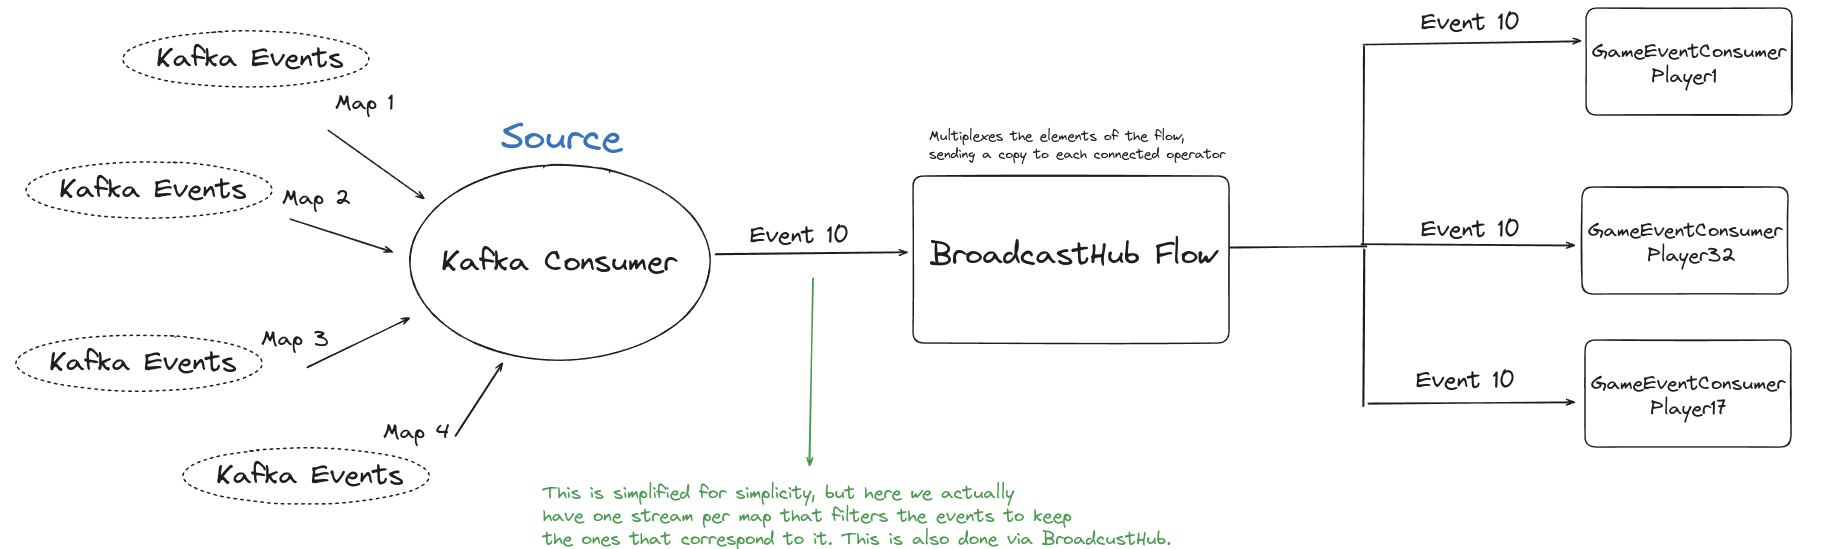
\includegraphics[width=1\textwidth]{../assets/kafka-consumer-flow.png}
    \caption{Pipeline de procesamiento de eventos del juego}
\end{figure}

Como último comentario, debido a que \textit{Fiubakka} hace uso de un único consumidor y productor de Kafka por nodo de la aplicación, se tendría un único punto de falla para ambos a nivel nodo.
Es decir, si el productor de Kafka en un nodo fallase, no se reportarían las acciones de los jugadores de dicho nodo al resto de los jugadores. De igual forma, si el consumidor de Kafka fallase, no
se enterarían los jugadores que residan en ese nodo de las acciones de todos los demás, si bien continuarían enviando sus propias acciones correctamente. En la práctica esto no introduce propiamente dicho un
único punto de falla en el servidor ya que es a nivel de nodo, por lo que no es tan crítico. Igualmente, es posible detectar el fallo y reintentar establecer la conexión del consumidor y productor con Kafka, por lo que
la caída del nodo sería temporal.

A continuación se provee una implementación resumida de los actores GameEventConsumer y GameEventProducer.

\begin{lstlisting}[language=Scala, caption={\textbf{Implementación del actor GameEventConsumer}}]
object GameEventConsumer {
    sealed trait Command extends CborSerializable
    
    def apply(
        player: ActorRef[Player.Command],
        partition: Int
    ): Behavior[Command] = {
        Behaviors.setup(ctx => {
            implicit val mat = Materializer(ctx)
            val playerId =
                player.path.name // The Player Entity Id is its Actor's name
        
            val playerSink: Sink[Player.Command, NotUsed] =
                ActorSink.actorRef(
                ref = player,
                onCompleteMessage = Player.GameEventConsumerFailure(
                    ctx.self,
                    "Stream completed when it's not supposed to"
                ),
                onFailureMessage = (error) =>
                    Player.GameEventConsumerFailure(ctx.self, error.getMessage())
                )
        
            KafkaConsumer(partition)
                .buffer(1024, OverflowStrategy.dropHead)
                .filter(record => {
                    (record.key == null || record.key != playerId)
                }) // Ignore messages from myself
                .map { record =>
                    ByteString(record.value)
                }
                .via(
                    InMessageFlow(
                        PBEventMetadata,
                        ProtocolMessageMap.eventConsumerMessageMap
                    )
                )
                .map { msg =>
                    Player.GameEventConsumerCommand(
                        eventCommandFromEventMessage(msg),
                        ctx.self
                    )
                }
                .instrumentedRunWith(playerSink)(
                    name = "GameEventConsumer",
                    reportByName = true
                )
        
            Behaviors.empty
        })
    }
}
\end{lstlisting}


\begin{lstlisting}[language=Scala, caption={\textbf{Implementación del actor GameEventProducer}}]
object GameEventProducer {
    sealed trait Command
    final case class PlayerStateUpdate(playerState: PlayerState) extends Command
    final case class AddMessage(msg: String) extends Command
    // This is actually also used anytime the Player should disappear from the map (ie. when starting a Truco match)
    final case class PlayerDisconnect() extends Command
    
    def apply(playerId: String, partition: Int): Behavior[Command] = {
        Behaviors.setup(ctx => {
            implicit val mat = Materializer(ctx)
            val gameZoneTopic =
                ctx.system.settings.config.getString("game.kafka.topic")
        
            val config = ctx.system.settings.config.getConfig("akka.kafka-producer")
            val producerSettings =
                ProducerSettings(config, new StringSerializer, new ByteArraySerializer)
                .withProducer(KafkaProducer())
        
            val (conQueue, conSource) = Source
                .queue[GeneratedMessage](1024, OverflowStrategy.dropHead)
                .preMaterialize()
        
            conSource
                .via(
                    OutMessageFlow(
                        (length: Int, `type`: GeneratedEnum) =>
                        PBEventMetadata(length, `type`.asInstanceOf[PBEventMessageType]),
                        ProtocolMessageMap.eventProducerMessageMap
                    )
                )
                .map(_.toArray)
                .map(value =>
                    new ProducerRecord(gameZoneTopic, partition, playerId, value)
                )
                .instrumentedRunWith(Producer.plainSink(producerSettings))(
                    name = "GameEventProducer",
                    reportByName = true
                )
        }
    }
}
\end{lstlisting}

\subsubsection{Sincronización inicial del jugador}

\noindent Mencionamos anteriormente que por motivos de practicidad y performance decidimos separar la persistencia del estado de la entidad Player en otro actor PlayerPersistor, el cual
es el que hace uso de los \textit{behaviors} de Durable State provistos en el módulo de Akka Persistence. Esta decisión conlleva que al momento de iniciar el Player no dispongamos ya del estado
inicial del jugador, sino que debemos esperar a que el PlayerPersistor nos lo envíe. Para manejar esta situación, el Player envía un mensaje al PlayerPersistor solicitando su estado inicial.
Se configura un \textit{timeout} esperado (al momento de este informe es de 30 segundos) como límite de tiempo para recibir la respuesta. En caso de error en el PlayerPersistor o que la respuesta no
nos llegue en el tiempo esperado, el Player se detendrá y notificará al PlayerHandler del error. El PlayerHandler luego notifica al cliente, y el cliente deberá reintentar iniciar sesión hasta que eventualmente
lo consiga. En la práctica estos casos únicamente comienzan a suceder cuando el sistema está bajo muchísima carga.

Por otro lado, el PlayerHandler deberá esperar también a que la entidad Player esté lista para poder confirmarle al cliente que la inicialización se completó correctamente. Al momento de su creación, el actor PlayerHandler
envía un mensaje a la entidad Player del tipo \textbf{Init}. Dado que Player es una entidad de Cluster Sharding, al recibir el mensaje se inicializará y realizará la sincronización correspondiente con el PlayerPersistor. En cuanto
haya obtenido el estado inicial así como también realizado la creación de sus correspondientes GameEventProducer y GameEventConsumer, contestará entonces al PlayerHandler el mensaje de \textbf{InitReady}, el cual completará la sincronización inicial
del cliente con su jugador en el servidor.

\begin{figure}[htbp]
    \centering
    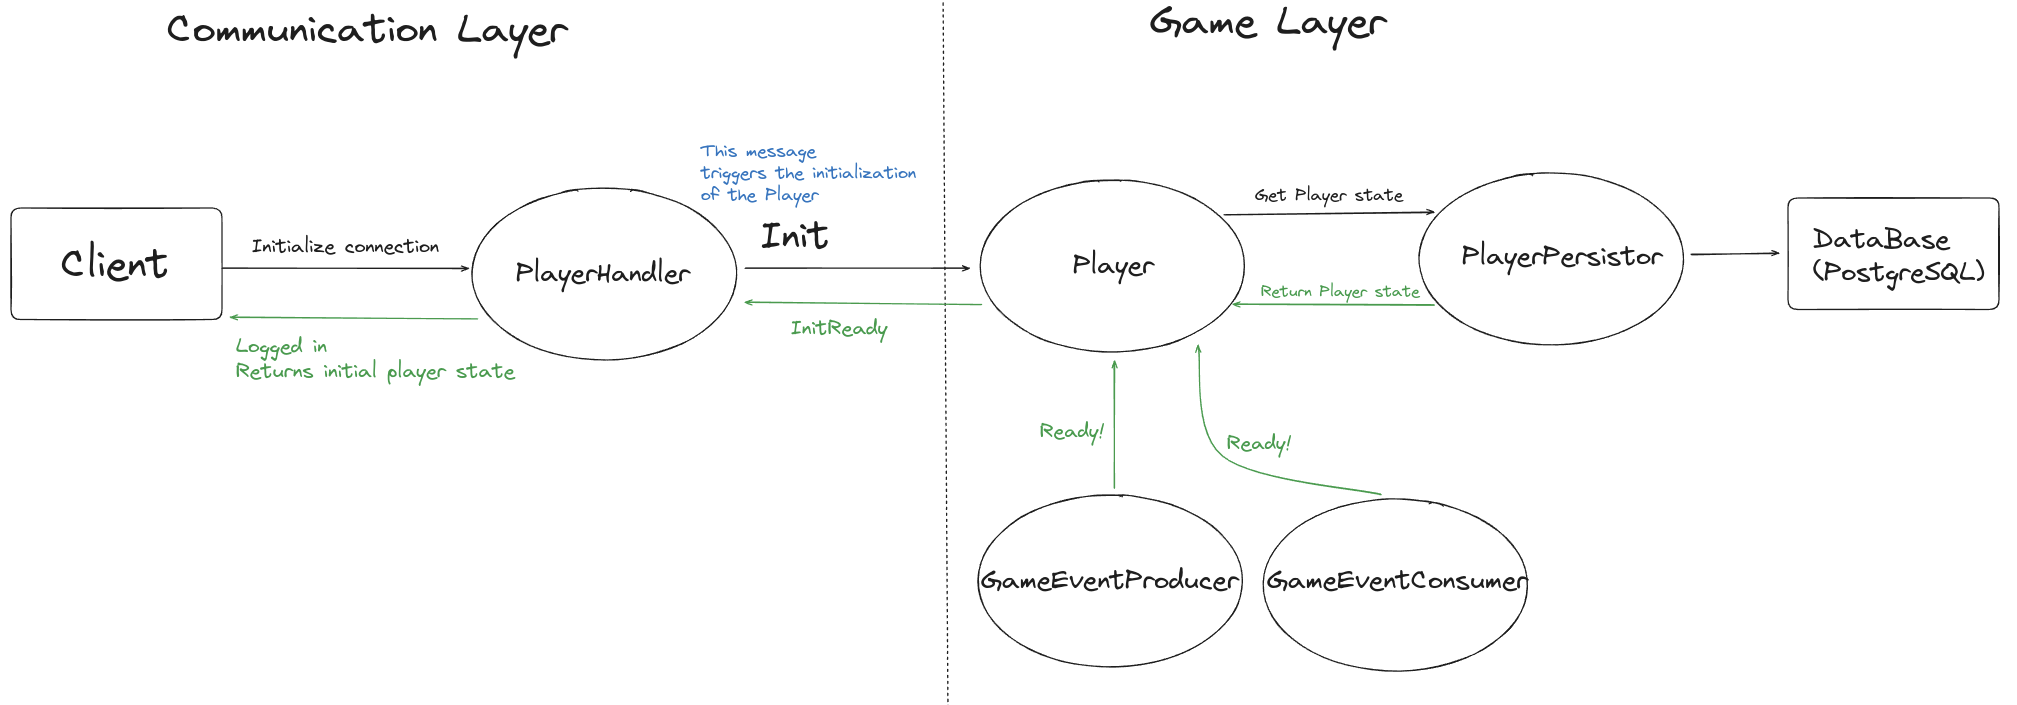
\includegraphics[width=1\textwidth]{../assets/player-init-sync.png}
    \caption{Flujo de sincronización inicial del jugador}
\end{figure}

La sincronización es ligeramente distinta cuando el jugador se registra, dado que el estado inicial lo proveerá el cliente en lugar del servidor. En dicho caso, el flujo es el siguiente.

\begin{figure}[htbp]
    \centering
    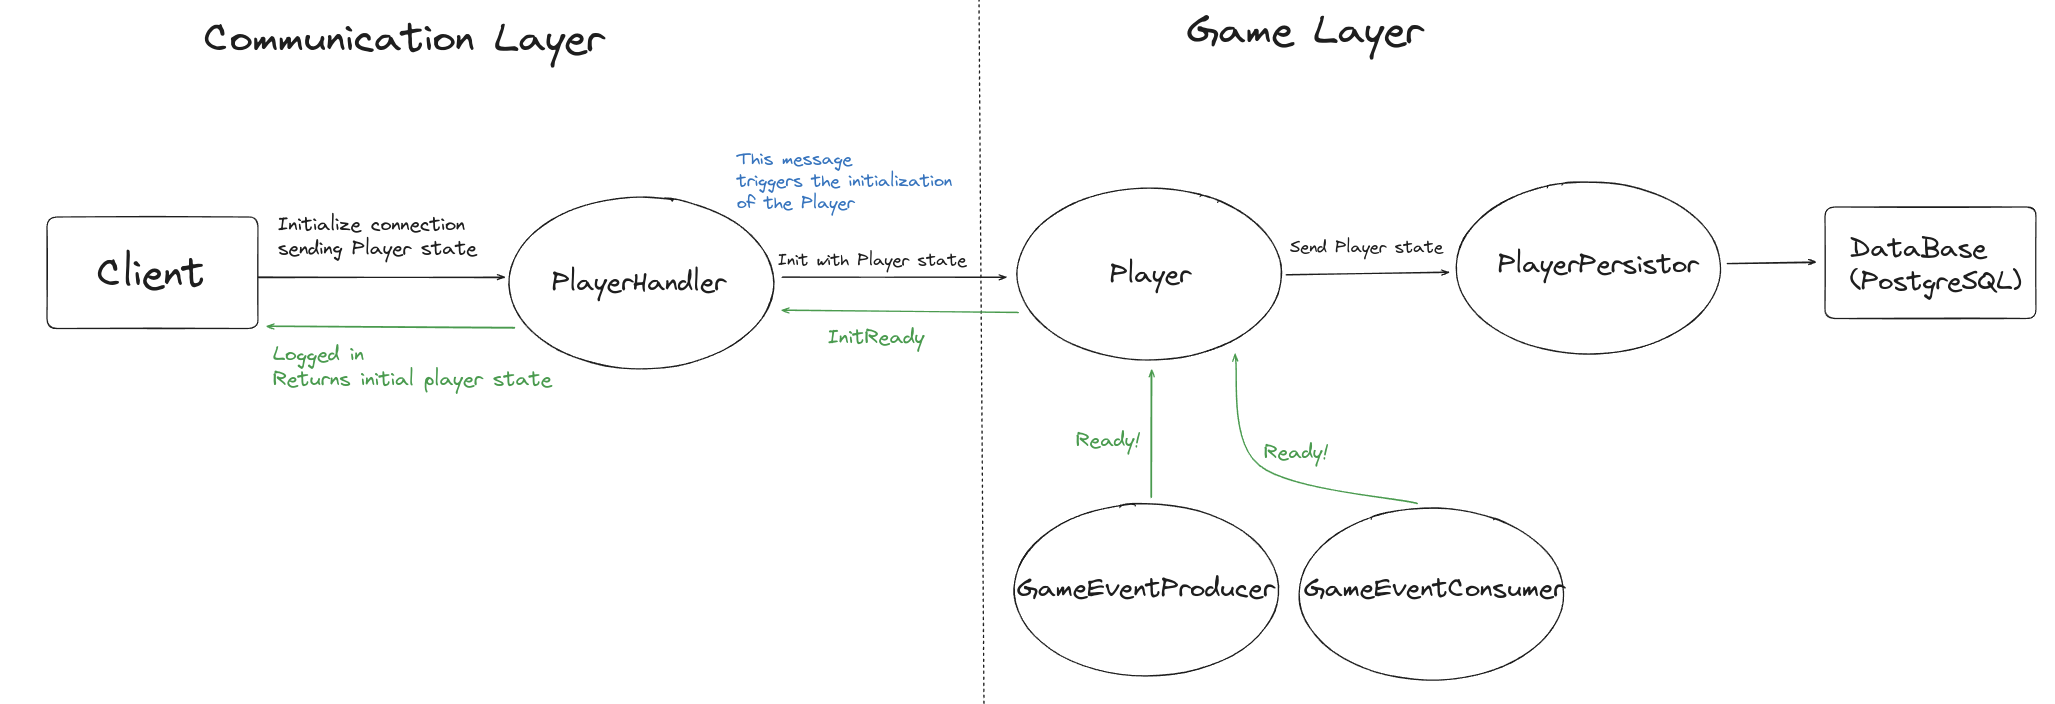
\includegraphics[width=1\textwidth]{../assets/player-init-register-flow.png}
    \caption{Flujo de registro del jugador}
\end{figure}

Vemos que ya no se hace un pedido del estado al PlayerPersistor dado que el mismo es provisto directamente por el cliente y recibido luego por el Player en el mensaje de \textbf{Init} del PlayerHandler.

\subsubsection{\textit{Heartbeats} del Player}

\noindent Se explicó en la sección de Cluster Sharding que las entidades de Akka son automáticamente pasivadas cada cierta cantidad de tiempo en el que no reciban ningún mensaje.
La intención detrás de este mecanismo es liberar recursos, dado que las entidades, a diferencia de los actores, son reiniciadas siempre que reciben un mensaje, por lo que no es práctico estar
deteniéndolas manualmente cuando no se las necesita. Una problemática que introduce nuestra arquitectura por el uso de entidades para el Player es que en caso de que la conexión con el cliente se corte y el Player
no reciba el mensaje correspondiente, la pasivación automática de Akka no entrará nunca en efecto. Esto se debe a que el GameEventConsumer continuará leyendo los distintos eventos que reciba desde Kafka, y seguirá enviándoselos
al Player. Dado que el Player nunca dejaría de recibir mensajes, la pasivación nunca se activaría. En la práctica, esto se conoce coloquialmente como un \textit{leak} de recursos.

Para solucionar este problema implementamos una técnica conocida como \textit{heartbeats}. Se trata de un mecanismo de mensajes periódicos entre los nodos de un sistema distribuido para asegurarse de que los componentes del sistema
siguen activos. Su uso es extremadamente común en los sistemas distribuidos, por ejemplo, Kubernetes lo utiliza para conocer el estado de los distintos nodos del cluster. Akka hace exactamente lo mismo para sus propios nodos del Akka Cluster.
\textit{etcd} es una base de datos distribuida que también lo emplea.

En nuestro caso, el PlayerHandler envía un mensaje de tipo \textbf{Heartbeat} hacia el Player cada 2 segundos. Cuando el Player recibe el mensaje actualiza un valor de su estado que indica el \textit{timestamp}
del momento en el que lo recibió. Adicionalmente, el Player se envía mensajes a sí mismo de forma periódica cada unos 5 segundos donde verifica si la diferencia entre el \textit{timestamp} actual y el almacenado en su estado
supera los 10 segundos. En caso de que así sea, el Player automáticamente da por perdida la conexión y se detiene, garantizando que los recursos se liberen.

\begin{figure}[htbp]
    \centering
    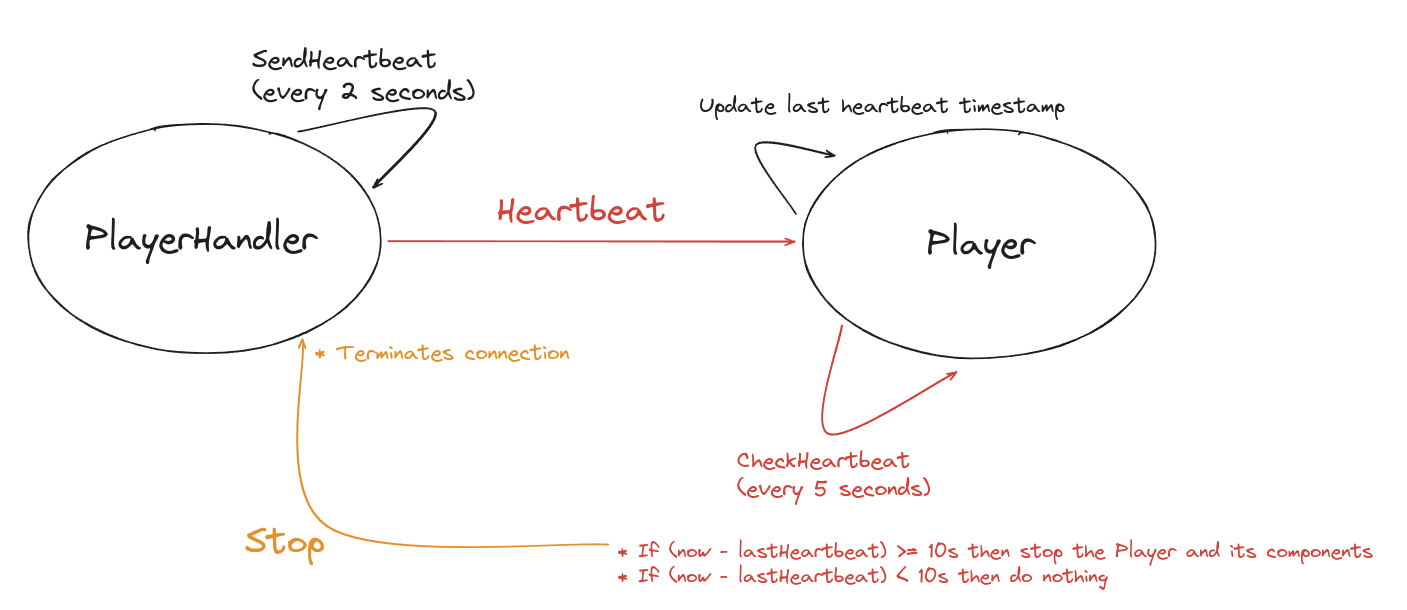
\includegraphics[width=1\textwidth]{../assets/player-heartbeat.png}
    \caption{Flujo de \textit{heartbeats} del Player}
\end{figure}

\newpage

Si la pasivación vía \textit{heartbeats} del Player se activa se envía además un mensaje de tipo \textbf{Stop} al PlayerHandler para que cierre la conexión. En la práctica este mensaje se envía por redundancia, dado que lo más probable
es que el PlayerHandler ya esté detenido si no recibimos ningún \textit{heartbeat} en los últimos 10 segundos.

\subsubsection{Rebalanceo del Player en el Akka Cluster}

\noindent Vimos que una de las principales ventajas de usar Akka Cluster Sharding es que permite el rebalanceo de entidades automáticamente al alterarse la composición de los nodos del Akka Cluster. Si bien es cierto que Akka se encargará de eliminar a una
entidad de un nodo e iniciarla nuevamente en otro de forma transparente, toda la lógica de sincronización de la capa de negocio es algo que debemos definir y manejar nosotros. Para el caso del Player, esto implica que al realizarse un reinicio de la entidad debemos 
volver a realizar la sincronización inicial del jugador. La diferencia principal que tenemos con el caso mostrado en la anterior sección es que el PlayerHandler no se entera de este rebalanceo, sino que sigue comunicándose con el Player normalmente.

Para poder recuperar el estado del Player únicamente debemos plantear un flujo distinto para la sincronización con el PlayerHandler. Al recibir cualquier mensaje del PlayerHandler el Player volverá a iniciarse (debido a las garantías de Cluster Sharding)
y volverá a solicitar su estado al PlayerPersistor e inicializar a su consumidor y productor de eventos del juego. El único punto faltante entonces sería recuperar la dirección del actor PlayerHandler para poder comunicarle los eventos del juego.
Sin embargo, el PlayerHandler desconoce que el Player necesita nuevamente su dirección, y sin su dirección, lógicamente, el Player no puede enviarle un mensaje pidiendole su dirección.

Es por esto que el mensaje de tipo \textbf{Heartbeat} contiene como argumento la dirección del PlayerHandler. Dado que sabemos que el PlayerHandler se encarga de enviar este mensaje periódicamente, tenemos la garantía de que eventualmente lo recibiremos.
El Player, en caso de recibir el mensaje de Heartbeat y estar en el \textit{behavior} de inicialización, almacenará la dirección del PlayerHandler en su estado y procederá a completar su inicialización. De aquí en adelante hemos recuperado el estado del Player
correctamente y el flujo de mensajes entre el Player y el PlayerHandler se reestablece.

Debido a que la fuente de la verdad del estado del jugador proviene del cliente, la próxima actualización de estado recibida garantizará la consistencia que se perdió durante el rebalanceo del Player.
Por supuesto, todo este proceso es transparente al cliente. Los únicos efectos generados por este proceso serían una breve inconsistencia entre lo que los demás jugadores ven que el jugador siendo rebalanceado está haciendo y lo que realmente el cliente que lo controla
hizo (por ejemplo, quedarse quieto en lugar de moverse).

\subsubsection{Bots}
\label{sec:Bots}

\noindent Para poder simular la presencia de múltiples jugadores en el juego y con el objetivo de hacer pruebas de carga es que
desarrollamos un actor \textbf{Bot}. Un bot, en la jerga de los videojuegos, es un \textit{mock} de un jugador que es en realidad controlado
por la computadora en lugar de una persona. En nuestro caso, el actor Bot reemplaza al actor PlayerHandler. Cuando el servidor se inicializa
lee la configuración de la cantidad de bots que debe iniciar y se encarga de crearlos. Una vez creado, el Bot crea su correspondiente entidad Player
y comienza a simular movimientos cada unos 16ms, lo que en la práctica es la máxima carga permitida por un jugador real.

Los movimientos realizados por los bots no siguen ningún tipo de patrón real, únicamente nos interesa que generen carga máxima sobre el sistema.
En el futuro, es posible implementarles lógica más compleja para simular comportamientos más realistas o hacer pruebas de carga más específicas.
En nuestros análisis de performance no nos interesamos tanto por los tipos de mensajes generados sino por la cantidad de actores y de mensajes que se estuvieran
procesando en un momento dado.

La implementación del Bot es sencilla. A continuación se muestra un extracto resumido de ella.

\begin{lstlisting}[language=Scala, caption={\textbf{Implementación del actor Bot}}]
object Bot {
    sealed trait Command
    private type CommandOrPlayerReply = Command | Player.ReplyCommand
    
    final case class RandomMove() extends Command
    final case class Heartbeat() extends Command
    
    final case class State(
        playerBot: EntityRef[Player.Command],
        position: Position
    )
    
    def runningBehavior(
        state: State
    ): Behavior[CommandOrPlayerReply] = {
        Behaviors.receive { (ctx, msg) =>
            msg match {
                case RandomMove() => {
                    // Generate random velocity with magnitude 1
                    val randVelocity = Velocity(2, 0)
                    val newPosition = Position(
                        state.position.x + randVelocity.x,
                        state.position.y + randVelocity.y
                    )
                    state.playerBot ! Player.Move(
                        velocity = randVelocity,
                        position = newPosition
                    )
                    runningBehavior(state.copy(position = newPosition))
                }

                case Heartbeat() => {
                    state.playerBot ! Player.Heartbeat(ctx.self)
                    Behaviors.same
                }
        
                case _ => Behaviors.same
            }
        }
    }
}
\end{lstlisting}

\subsubsection{Resumen de la arquitectura}

\noindent En las anteriores secciones ahondamos en los distintos componentes que integran a \textit{Fiubakka} y las relaciones entre ellos. Partimos de los conceptos esenciales
de Akka y mostramos qué papel juega cada uno de ellos en nuestra aplicación. A modo de resumen y para tener una vista más panorámica de la arquitectura, el siguiente diagrama engloba
todos los conceptos explicados hasta ahora. Si bien \textit{Fiubakka} cuenta con algunos features más que mostraremos en las posteriores secciones, lo descrito hasta ahora es el
núcleo de la aplicación.

\begin{figure}[htbp]
    \centering
    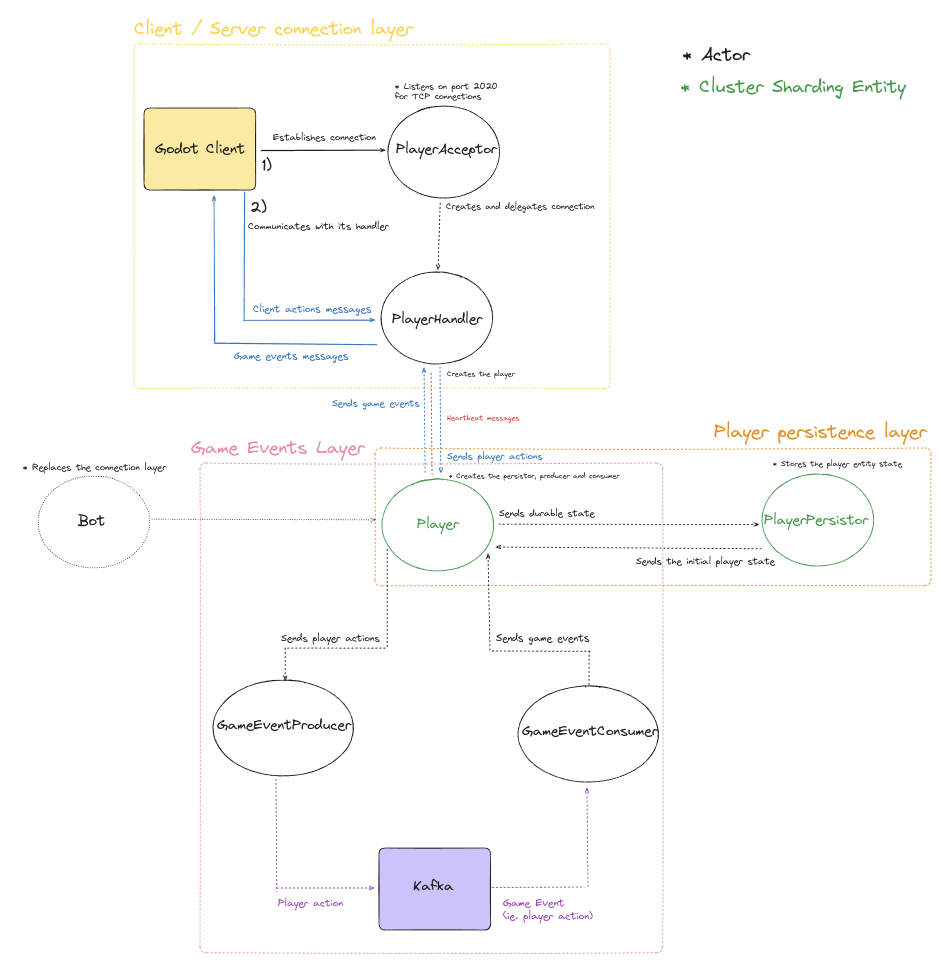
\includegraphics[width=1\textwidth]{../assets/fiubakka-architecture.png}
    \caption{Arquitectura núcleo de Fiubakka.}
\end{figure}

\newpage

\subsection{Truco: un minijuego dentro de Fiubakka}

\noindent Hasta aquí llega la explicación de la arquitectura \textit{core} de \textit{Fiubakka}. Si bien implementamos varios features dentro de Fiubakka para experimentar con lo que es posible hacer
en nuestro videojuego (como puede ser la sala de chat, las transiciones entre distintos mapas o la posibilidad de cambiarse el equipamiento mediante el inventario) el \textit{feature} principal
que implementamos es el \textit{Truco}, el juego de cartas más famoso de Argentina.

La arquitectura utilizada en el desarrollo del Truco puede ser aplicada a cualquier otro juego de cartas entre cualquier cantidad de personas dentro de \textit{Fiubakka}.
A diferencia de los eventos del juego, los cuales son transmitidos a través de Kafka y recibidos por el GameEventConsumer de cada Player, los mensajes del Truco son enviados directamente entre las entidades
y actores involucrados en el juego. Esto se debe a que son mensajes que únicamente le son de interés a un número muy reducido de actores, por lo que no se trata de eventos masivos y no es necesario enviarlos por Kafka.

\subsubsection{Inicio de partida de Truco}

\noindent En primer lugar el cliente debe solicitar al servidor que desea iniciar una partida de Truco con otro jugador. En el mensaje de solicitud es únicamente requerido como argumento el nombre de usuario del jugador
con el que desea entablar una partida. Esa información es siempre enviada al cliente cuando se procesan los eventos del juego, por lo que ya la tiene disponible. En el momento en el que el servidor recibe la solicitud de inicio
de partida, le envía al cliente del jugador desafiado un mensaje de notificación mostrándole quién lo desafió y dándole la opción de aceptar o rechazar el desafío. En caso de que el jugador desafiado rechace el desafío,
se desestima la partida. Si, por otro lado, el desafío fue aceptado, se procede de la siguiente forma.

El Player que aceptó el desafío crea un actor \textbf{TrucoManager} que se encargará de administrar la lógica de la partida y notificar a los jugadores involucrados. El TrucoManager enviará un mensaje de tipo
\textbf{SyncTrucoMatchStart} a ambas entidades Player que participan en la partida. Este mensaje recibirá como respuesta un \textbf{PlayerSyncedTrucoMatchStart} con el nombre del jugador que ya está listo para comenzar a jugar.
Una vez que ambos jugadores estén listos, comienza la partida.

\newpage

\begin{figure}[htbp]
    \centering
    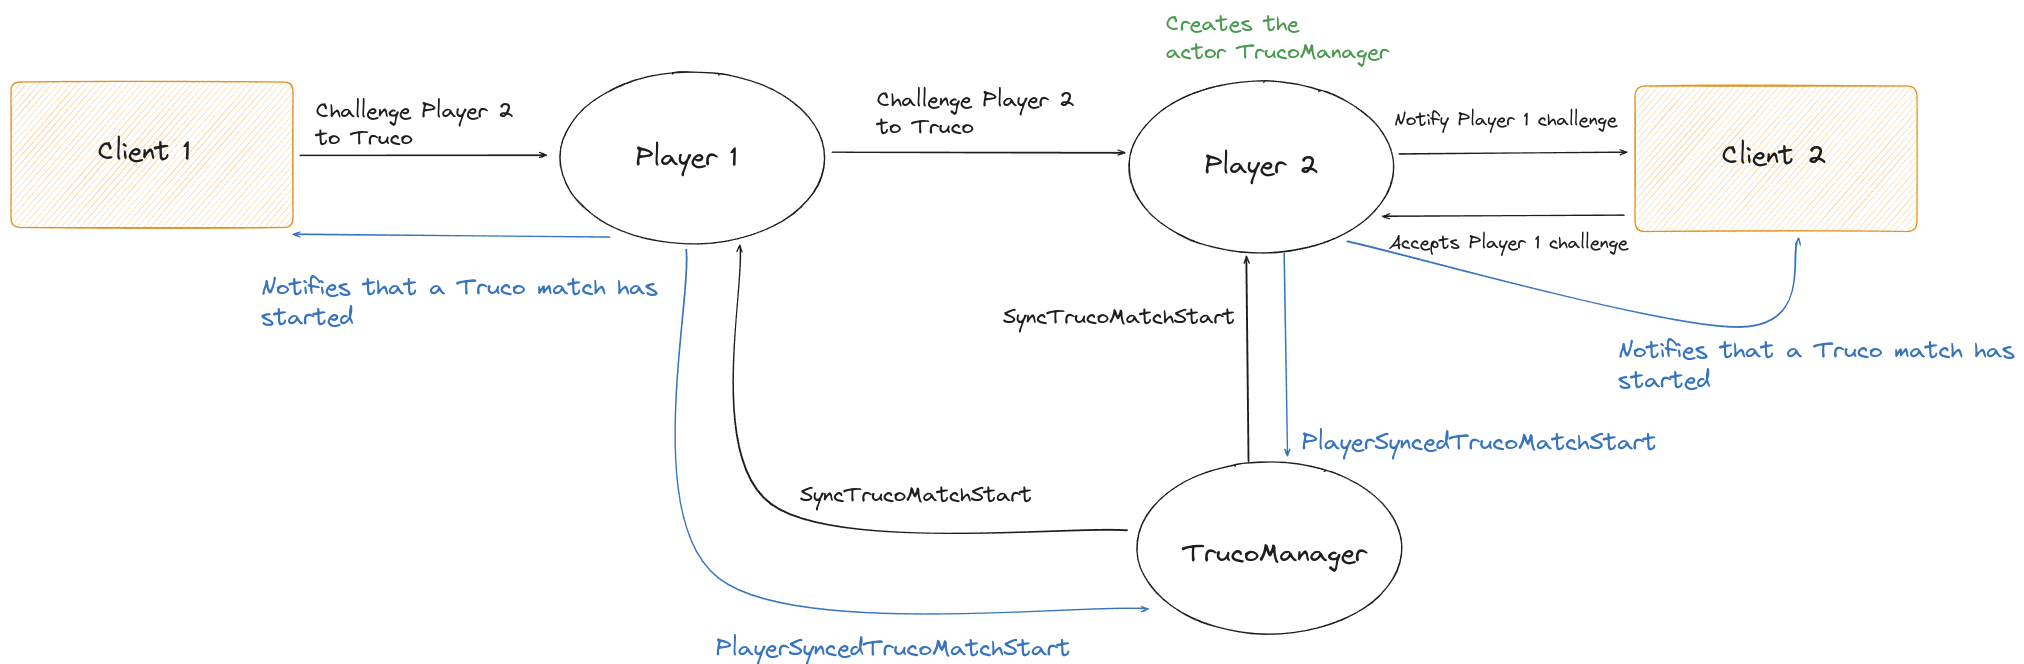
\includegraphics[width=1\textwidth]{../assets/truco-match-init.png}
    \caption{Sincronización inicial de partida de Truco}
\end{figure}

En la figura anterior no se muestran los PlayerHandler para simplificar el flujo, pero por supuesto siempre están presentes como capa intermedia entre el cliente y su correspondiente entidad Player.

\subsubsection{Protocolo de comunicación del Truco}

\noindent Una vez comenzada la partida de Truco el TrucoManager inicializa los modelos de dominio del juego, los cuales manejarán la lógica de las actualizaciones y mantendrán el estado central
de la partida. A diferencia de la arquitectura \textit{core} de \textit{Fibuakka}, que vimos que es descentralizada, el estado del Truco se encuentra centralizado en una clase \textbf{TrucoMatch}, que es
administrado por el actor TrucoManager. Cada partida de Truco tendrá su correspondiente TrucoManager asociado, es decir, son independientes entre sí. El motivo por el que el estado de la partida de Truco debe ser centralizado se debe principalmente a los siguientes puntos:

\begin{itemize}
    \item Dado que una partida de Truco típica se compone por dos jugadores, mantener una copia del juego en cada jugador podría resultar en desincronizaciones entre ambos que no habría forma de conciliar.
    \item Mantener estado centralizado en el servidor evita posibles trampas, esencial en juegos competitivos.
    \item No hay ventajas prácticas en descentralizar el estado de la partida.
\end{itemize}

Dado que el estado se encuentra centralizado en el servidor es necesario asegurarnos que los jugadores tengan el estado correcto reflejado en cada cliente para poder avanzar correctamente con el desarrollo de la partida.
Además debemos tomar en cuenta que todo mensaje enviado por el cliente al servidor o viceversa puede perderse, debido a la naturaleza del modelo de actores. En general, esta característica del modelo de actores no resulta
en un problema en el resto del juego porque justamente está diseñado alrededor de la consistencia eventual y el tipo de juego desarrollado no requiere sincronización entre todos los clientes para funcionar correctamente. Para el caso
del Truco (o cualquier otro juego de cartas) es necesaria la \textbf{consistencia inmediata}, es decir, no podemos avanzar en el juego hasta tanto no nos hayan confirmado todos los jugadores que estén sincronizados con el último estado del juego.

Para garantizar la sincronización constante entre los clientes y el estado del Truco en el servidor decidimos utilizar un protocolo de \textit{acknowledgements} ante cada cambio de estado de la partida. A cada cambio,
como por ejemplo al realizar una jugada o al transicionar de ronda, se le asocia un identificador numérico incremental llamado \textbf{playId} y se envía la actualización a los clientes. Esta notificación se realiza periódicamente para evitar problemas devenidos por la
pérdida de mensajes inherente en los actores. Cuando el cliente recibe la notificación de cambio de estado, revisa si el \textbf{playId} recibido es el siguiente al almacenado por él. En caso de serlo, aplica la actualización a su partida y envía
un mensaje de \textit{acknowledgement} al servidor con el \textbf{playId} recibido. El servidor esperará a recibir la confirmación de ambos jugadores para poder pasar a la siguiente jugada o estado del juego, según correspondiese.

Si el servidor determina que es el turno de alguno de los jugadores en hacer una jugada, les enviará un mensaje de notificación indicándoles que es su turno de jugar y que está a la espera de su jugada. Lógicamente, este mensaje también se enviará
periódicamente hasta que reciba la jugada del jugador correspondiente. El cliente, al recibir el mensaje de habilitación de jugada, enviará la jugada realizada también de forma periódica hasta que reciba el mensaje de actualización del juego desde el servidor,
con el \textbf{playId} siguiente que corresponda.

Este protocolo garantiza que ambos clientes estén sincronizados con el estado del juego en todo momento, evitando problemas ocasionados por la pérdida de mensajes u orden de los mensajes recibidos. Garantizar la sincronización constante nos permite además optimizar el tamaño
de los mensajes enviados, ya que solo necesitamos notificar el cambio (por ejemplo, carta jugada por el rival) en lugar de notificar el estado completo de la partida ante cada cambio. 

\newpage

\begin{figure}[htbp]
    \centering
    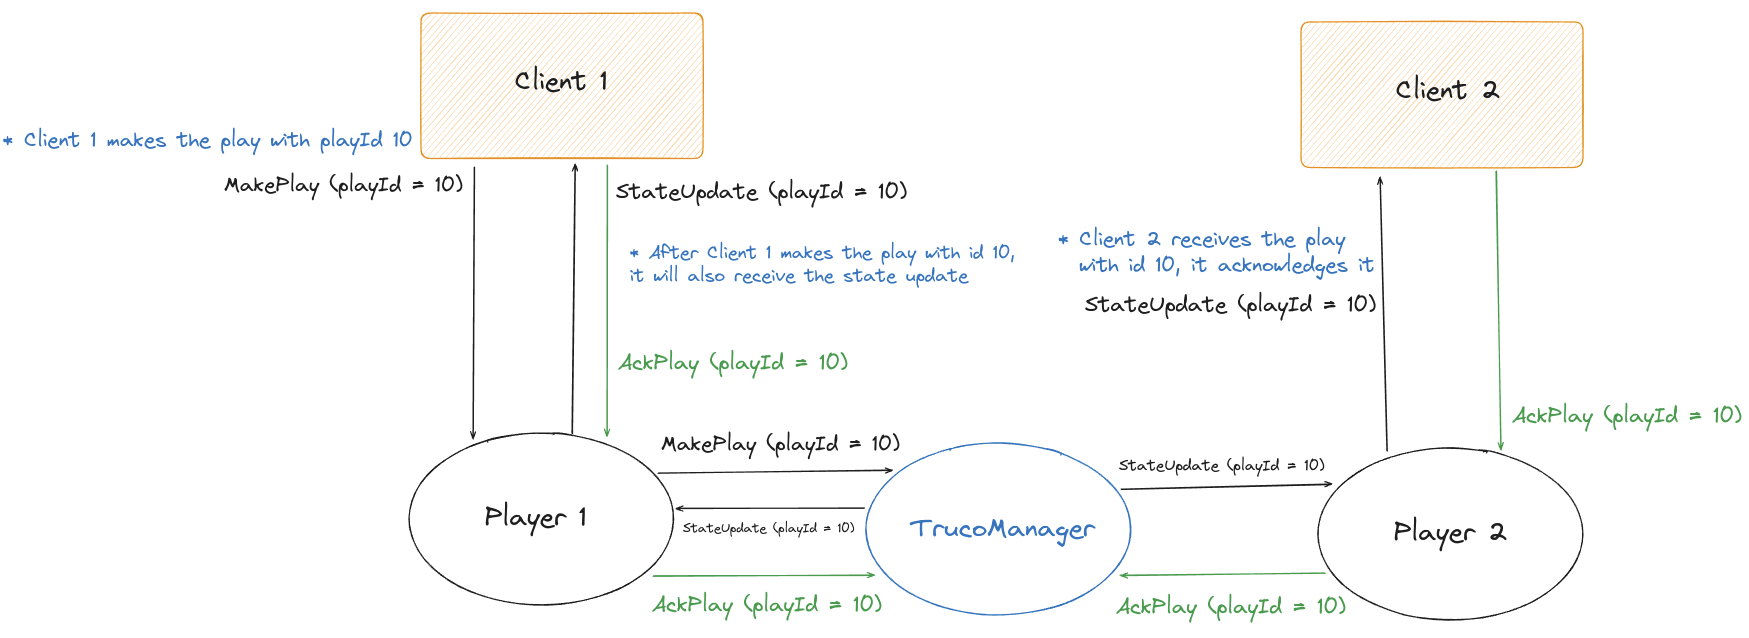
\includegraphics[width=1\textwidth]{../assets/truco-state-update.png}
    \caption{Diagrama de flujo de jugada en el Truco.}
\end{figure}

\subsubsection{Fin de partida de Truco}

\noindent Una vez que la partida de Truco finaliza, ya sea porque uno de los jugadores cumplió con el objetivo de puntos o abandonó, es necesario notificar a ambos clientes que la partida ha terminado y retornar el estado del Player al previo a comenzar la partida de Truco.
En el caso de que la partida termine porque uno de los jugadores ganó, el TrucoManager lo indicará en el mensaje de actualización de estado del juego a ambos clientes. Al recibirlo, el cliente enviará el mensaje de tipo \textbf{TrucoDisconnect}. La entidad Player volverá
al comportamiento normal de procesar eventos del juego y se lo notificará al cliente mediante el mensaje \textbf{TrucoDisconnectAck}, el cual es un mensaje de \textit{acknowledgement} de desconexión del Truco. El cliente deberá reenviar el mensaje de desconexión periódicamente hasta
que reciba dicho mensaje de confirmación, esto evita situaciones de desincronización entre el cliente y el servidor.

En el caso de que la partida termine porque uno de los jugadores abandonó, el TrucoManager lo detectará y enviará un mensaje de tipo \textbf{TrucoPlayerDisconnected} al jugador que todavía está en la partida, de forma periódica al igual que en el caso anterior. Al recibir este mensaje,
el cliente enviará el mensaje de \textbf{TrucoDisconnect} y se repite el flujo descrito para el anterior caso. De esta forma logramos volver al juego principal y mantener al cliente sincronizado con el servidor.

\newpage

\begin{figure}[htbp]
    \centering
    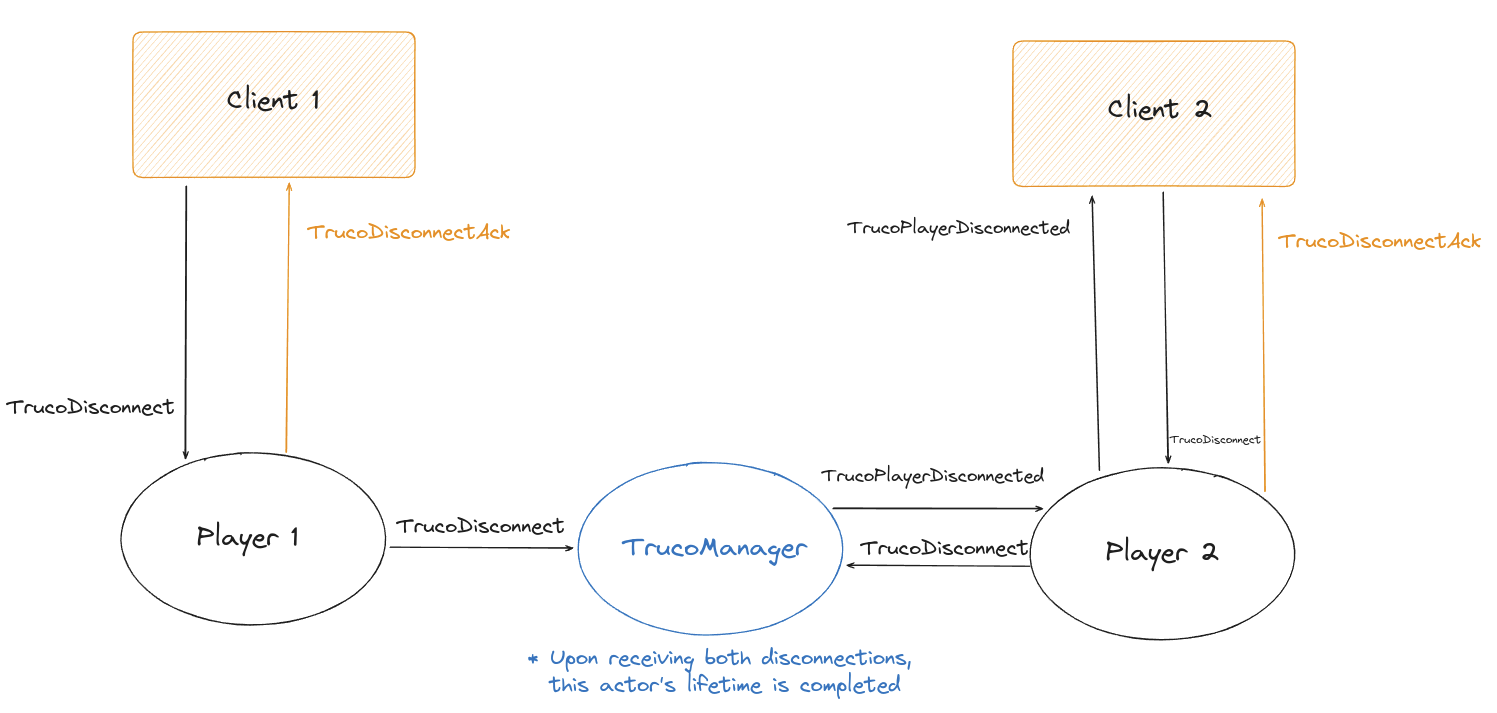
\includegraphics[width=1\textwidth]{../assets/truco-disconnection.png}
    \caption{Diagrama de desconexión de partida de Truco al abandonar un jugador.}
\end{figure}

\subsection{Protocolo de comunicación}
\label{sec:communication-protocol}

\noindent Tanto la comunicación por TCP entre cliente y servidor así como el envío de eventos con Kafka
requirió que definamos un protocolo de mensajes propio. Este protocolo lo diseñamos con el objetivo de
que sea rápido y eficiente, para mantener al mínimo la latencia entre mensajes y poder maximizar el \textit{throughput}.
Es por esto que decidimos usar \textit{Protocol buffers} (o \textit{protobufs}), un formato de serialización de data estructurada
desarrollado por Google que se caracteriza por su bajo consumo de memoria y eficiencia de serialización.
Cuenta con un lenguaje propio para definir los mensajes e implementaciones ya desarrolladas por la comunidad para su integración
con diversos lenguajes y tecnologías.

Los mensajes del protocolo los definimos en un repositorio central que es consumido por el cliente y el servidor, por lo que cualquier cambio
en la estructura del mensaje genera el recompilado correspondiente en cada uno.
Otra de las razones por la cual elegimos usar esta herramienta fue que cuenta con soporte tanto para Scala como para Godot.
Esto nos permitió que, una vez definidos los mensajes en sus correspondientes archivos \textit{.proto}, podamos usarlos
directamente en el código como si fueran objetos y al momento de compilar la apliación se los serializa automáticamente.

El formato de todos los mensajes consiste en una sección de metadata y otra sección que contiene el contenido del mensaje específico,
más dos campos de 4 bytes cada uno que indican el largo (en bytes) total del mensaje y el de la sección de metadata.
La metadata contiene dos valores: el largo del contenido, en 4 bytes, y el tipo de mensaje enviado.

\begin{figure}[htbp]
    \centering
    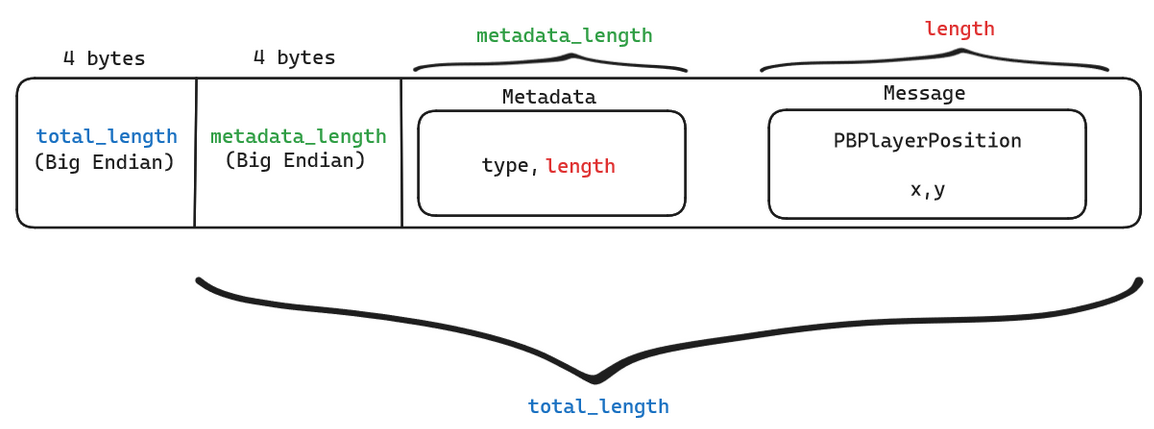
\includegraphics[width=1.0\textwidth]{../assets/protobuf.png}
    \caption{Estructura de un mensaje serializado.}
\end{figure}

\newpage

Todo mensaje enviado pasa por el siguiente proceso. En primer lugar, creamos un objeto que tenga el formato correspondiente a alguno de los
mensajes definidos. Luego, lo serializamos con el método correspondiente de protobuf (según estemos en Scala o Godot) y
calculamos la cantidad de bytes que ocupa el mensaje serializado. En base al tipo de mensaje y su tamaño serializado es que formamos el objeto de metadata, incluyendo el largo calculado y el tipo.
Finalmente, serializamos la metadata, le concatenamos el mensaje serializado original y anteponemos tanto el largo del mensaje total como el de la metadata.
Llegado este punto ya tenemos la totalidad del mensaje serializado y estamos listos para enviarlo por el canal correspondiente.

Para leer un mensaje recibido el flujo es el contrario. Leemos los primeros 4 bytes que nos indican el largo
total del mensaje, y procedemos a leer el mensaje total. Luego, con el mensaje leído y almacenado en un \textit{buffer}, leemos los primeros 4 bytes que nos indican el tamaño que ocupa la metadata. Con esta información, podemos leer
el campo de metadata, que a su vez nos indica el tipo y el largo del contenido del mensaje en sí. Finalmente, al saber el tipo del contenido, lo
deserializamos para luego poder manejarlo correctamente.

Los mensajes de contenido están definidos en archivos \textit{.proto}. Por ejemplo, veamos el siguiente
mensaje que definimos para el movimiento de un jugador:

\begin{lstlisting}[language=protobuf]
syntax = "proto2";

package protobuf.client.movement;

message PBPlayerVelocity {
    required float x = 1;
    required float y = 2;
}

message PBPlayerPosition {
    required float x = 1;
    required float y = 2;
}

message PBPlayerMovement {
    required PBPlayerVelocity velocity = 1;
    required PBPlayerPosition position = 2;
}
\end{lstlisting}

El mensaje que el cliente enviará es \textbf{PBPlayerMovement}, que incluye otros dos mensajes:
\textbf{PBPlayerVelocity} y \textbf{PBPlayerPosition}, ambos vectores bidimensionales representados
por sus coordenadas en \textbf{x} e \textbf{y}. De esta forma cuando el usuario controla y mueve a
su personaje, el cliente se lo comunica al servidor creando una instancia de \textbf{PBPlayerMovement}
con los valores correspondientes, serializándolo y finalmente enviándolo.

La totalidad de los mensajes que definimos en nuestro protocolo pueden encontrarse en el Anexo \ref{apendix:protobuf}.

\subsection{Ambiente productivo: Kubernetes}
\label{sec:kubernetes}

\noindent Todas las propiedades de escalabilidad de Akka pierden su valor si no se cuenta con un ambiente que permita administrar la configuración del cluster
de forma automática y se encargue de reemplazar las instancias del servidor que fallen o permita escalar dinámicamente la configuración de nodos del cluster.
Naturalmente, \textbf{Kubernetes} surge como la solución ideal donde desplegar una aplicación basada en Akka, y es por esto que decidimos utilizarlo para nuestro ambiente productivo.

Kubernetes es un sistema de orquestación de contenedores \textit{open source} que permite automatizar el despliegue, escalamiento y manejo de aplicaciones de \textit{software}.
Dado que Akka y Kubernetes son tecnologías que se complementan perfectamente, existe un \textit{plugin} de Akka llamado \textbf{Akka Management} especialmente orientado a los despliegues
en Kubernetes. Cuando la aplicación se ejecuta en un cluster de Kubernetes e inicializa el módulo de Akka Management, se levanta por un lado un servidor HTTP donde se pueden recibir \textit{requests}
de otros nodos que deseen unirse al cluster de Akka. En paralelo, el mismo nodo se encarga de hacer un \textit{discovery} en el ambiente de Kubernetes de otros nodos que estén inicializados y deseen formar
un cluster. Cuando los nodos se descubren entre sí, se ponen de acuerdo en quién será el líder del Akka Cluster y comienzan a formar el cluster. Particularmente, la elección de líder en Akka es un algoritmo determinístico,
es decir, dado un conjunto de nodos siempre se elegirá al mismo líder.

Si un nodo del Akka Cluster falla, el líder se encarga de eliminarlo del cluster y notificar a los demás miembros. Si el líder es el que falla, automáticamente los demás miembros saben que el siguiente líder
es el nodo más antiguo registrado en el cluster. Kubernetes, al detectar el fallo del nodo, se encargará de crear una nueva instancia para mantener la cantidad de réplicas de la aplicación constante según el valor
configurado. La nueva instancia se unirá al cluster; efectivamente recuperándose el sistema sin necesidad de intervención humana.

El proceso descrito anteriormente ignora la configuración de \textit{seed nodes} descrita en la sección \ref{config:akka-cluster}, ya que el descubrimiento de los demás nodos es dinámico y no se cuenta
con IPs estáticas.

Respecto al proveedor de Kubernetes, \textit{Fiubakka} no utiliza ningún proveedor Cloud; se encuentra desplegado de forma totalmente \textit{self hosted} en un cluster de RaspberryPis administrado
por uno de los integrantes del equipo. Tanto Kafka, PostgreSQL, el servidor de \textit{Fiubakka}, como todos los demás componentes necesarios para el correcto funcionamiento y monitoreo del servidor se ejecutan en este cluster.
En la sección \ref{sec:lessons-kubernetes} se encuentra la explicación del por qué fuimos por esta solución y las ventajas que nos brindó.

\begin{figure}[htbp]
    \centering
    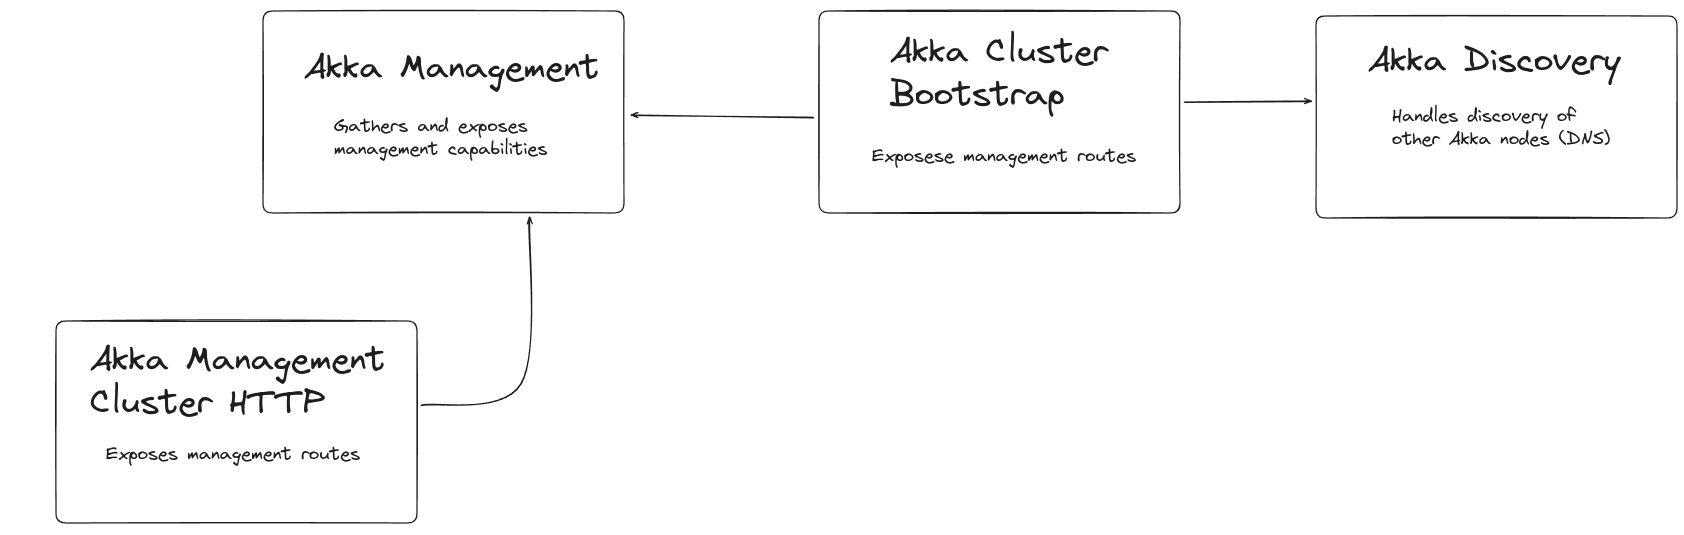
\includegraphics[width=1\textwidth]{../assets/akka-management.png}
    \caption{Componentes del \textit{discovery} de nodos de Akka en Kubernetes.}
\end{figure}

Con esto concluimos todo lo que compete al servidor de \textit{Fiubakka}. En las siguientes secciones analizaremos la otra columna de nuestro proyecto: el cliente de Godot.

\subsection{Cliente: Godot}

\noindent \textit{Godot} es un motor para desarrollo de videojuegos, de origen argentino, gratuito y de código abierto. 
Fue creado originalmente en 2001 por Juan Linietsky y Ariel Manzur para su propio estudio de juegos,
y luego se hizo público en 2014, bajo la licencia MIT. Godot recibió una gran cantidad de apoyo y funcionalidades desde su 
lanzamiento \textit{open source}.

Este motor brinda distintas herramientas para desarrollar aplicaciones interactivas (principalmente
videojuegos), como por ejemplo interfaces gráficas, gráficos 2D y 3D, input del usuario con distintos periféricos, 
control de audio, lógica de físicas y colisiones, conectividad a través de la red, entre muchas otras.
Además de permitir desarrollar para múltiples plataformas, permite programar scripts exponiendo una 
API orientada a objetos en los lenguajes C++, C\# e incluso GDScript, un lenguaje propio de Godot. 

\begin{figure}[htbp]
    \centering
    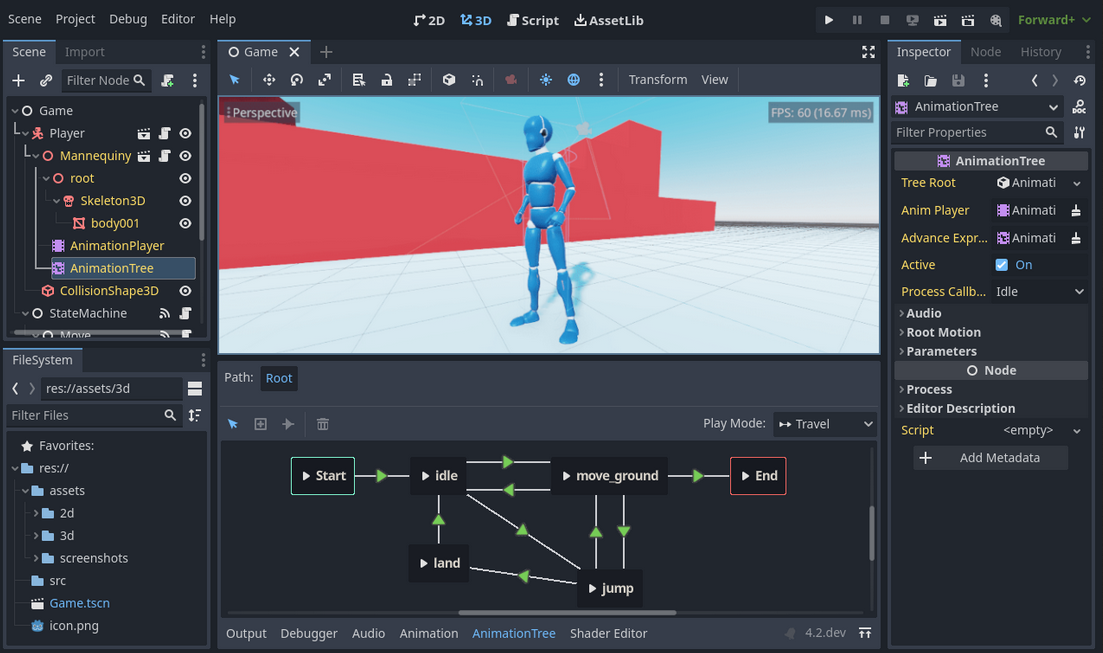
\includegraphics[width=1.0\textwidth]{../assets/godot-engine-showcase.png}
    \caption{Editor de Godot Engine \cite{ref1}.}
\end{figure}

\textit{GDScript} es un lenguaje de programación interpretado de alto nivel y con sintaxis similar a Python. 
El hecho de que sea un lenguaje interpretado tiene la ventaja de que no es necesario volver a compilar 
todo el código cada vez que se hacen modificaciones sobre el mismo.
A partir de la versión 4.0 de Godot, GDScript ofrece soporte opcional de tipado estático, el cual puede
mejorar la performance en las \textit{builds} de desarrollo, mejora la productividad del desarrollo al eliminar los errores
de tipos y aumenta la eficiencia del código.

\begin{figure}[htbp]
    \centering
    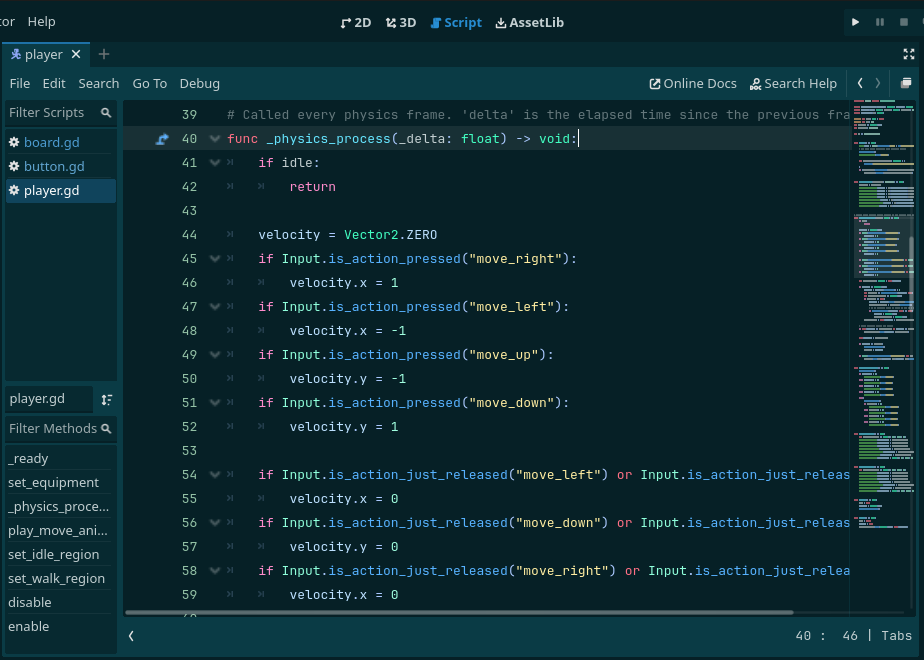
\includegraphics[width=0.8\textwidth]{../assets/godot-code-editor.png}
    \caption{Editor de código de Godot.}
\end{figure}

\newpage

El motor ofrece una amplia colección de \textbf{Nodos}, que son los componentes básicos que se utilizan para 
construir \textbf{Escenas}. A su vez, estas escenas pueden ser sub-nodos de otras escenas. Los Nodos pueden ser desde un 
simple botón hasta un cuerpo tridimensional con lógica de físicas y colisiones 
e incluso un \textbf{AnimationPlayer} que se encarga de manejar animaciones, 
es decir, una secuencia de imágenes o \textit{sprites}.

Estos Nodos poseen distintos atributos que se pueden configurar y modificar según se desee.
No solo eso, sino que además se les puede añadir un script, extendiendo y personalizando
su comportamiento como sea necesario.

\begin{figure}[htbp]
    \centering
    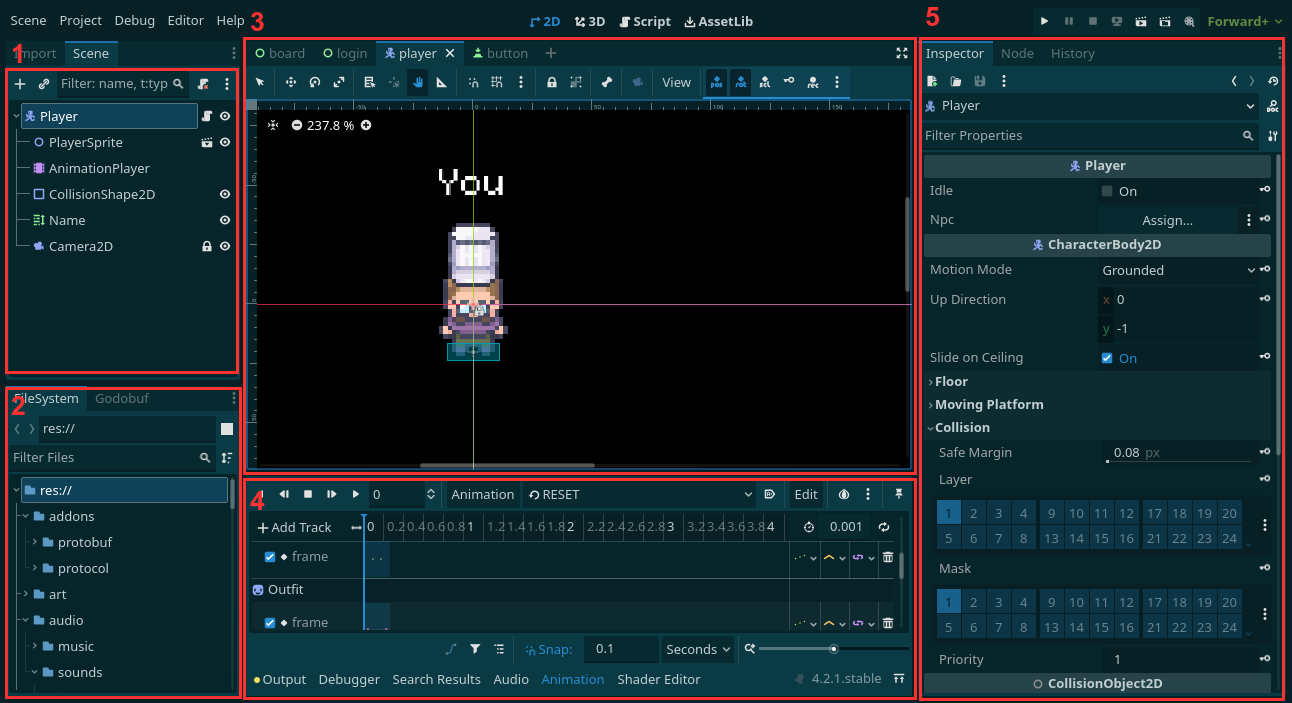
\includegraphics[width=1.0\textwidth]{../assets/godot-editor.png}
    \caption{Interfaz gráfica del editor de Godot. Los componentes enumerados son: el árbol de nodos (1),
            el explorador de archivos (2), el editor de la escena (3), el panel de animaciones (4) y el
            inspector del nodo seleccionado (5).}
\end{figure}

\newpage

Otro feature importante de Godot es el uso de señales (\textit{signals}) para comunicar eventos entre nodos.
Tanto los Nodos por defecto como las Escenas compuestas personalizadas pueden emitir \textit{signals} con un nombre específico 
(e incluso con parámetros) para que otros Nodos o Escenas se suscriban a dicha señal. Al suscribirse, los 
Nodos receptores definen un \textit{handler} para manejar 
la señal recibida. De esta forma se pueden crear escenas compuestas de múltiples Nodos distintos, con 
comportamiento más complejo, pero sin acoplar todos los nodos que necesiten comunicarse entre sí. En la
Figura \ref{fig:signals-editor} se ejemplifica cómo se ve una señal en el editor de Godot. Cuando el nodo LoginUsername emite la signal
username\_submitted, el nodo Login la recibe en su función \textit{\_on\_login\_username\_text\_submitted}. Por otro lado,
la Figura \ref{fig:signals-diagram} ilustra cómo es el flujo al emitirse una señal. Primero se define la señal text\_submitted
en el nodo LoginUsername y se la conecta al nodo Login (que es padre de LoginUsername).
Al emitirse esta señal, Login la escucha y entonces ejecuta su función handler
\textit{\_on\_login\_username\_text\_submitted}.

\newpage

\begin{figure}[htbp]
    \centering
    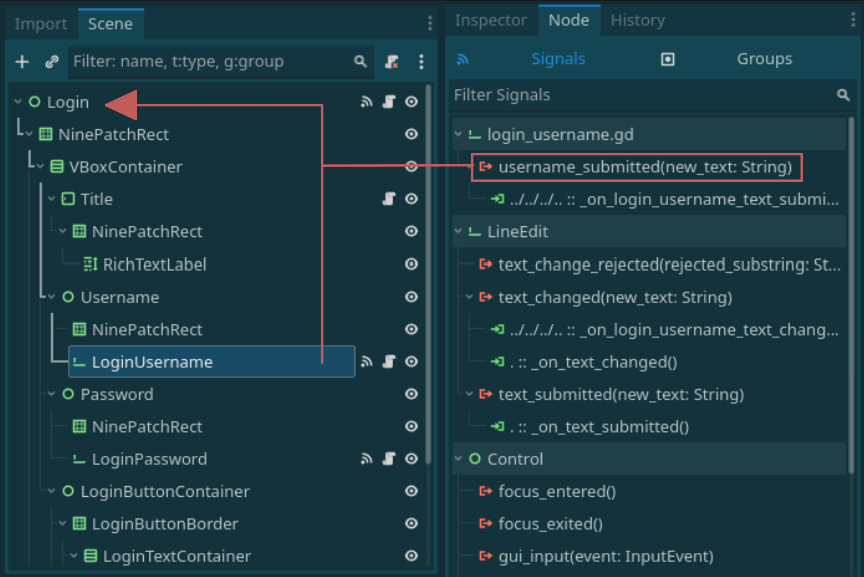
\includegraphics[width=0.7\textwidth]{../assets/godot-signals.png}
    \caption{Ejemplo de conexión de una signal.}
    \label{fig:signals-editor}
\end{figure}

\begin{figure}[htbp]
    \centering
    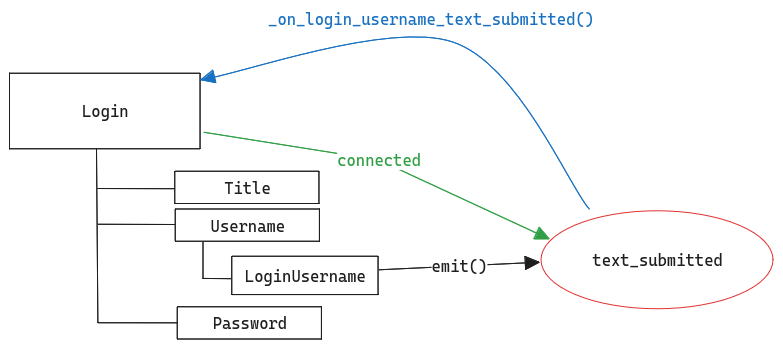
\includegraphics[width=0.7\textwidth]{../assets/godot-signals-diagram.png}
    \caption{Diagrama del flujo de emisión de una signal.}
    \label{fig:signals-diagram}
\end{figure}

La filosofía del diseño de Godot es construir Escenas reutilizables usando Nodos. A estas escenas y 
nodos se les puede agregar comportamiento con \textit{scripts}. Con la composición y jerarquía de los Nodos, 
se puede construir una lógica de juego que es clara y fácil de entender.
Es por estas características de cohesión, simplicidad y eficiencia en el diseño de Godot, así
como también el tipo de herramientas que provee, que optamos por usar este motor para el desarrollo del
cliente del proyecto en lugar de crear módulos de autoría propia con un lenguaje de más bajo nivel, 
como por ejemplo C o C++.

\subsubsection{Estructura de proyecto}

\noindent A continuación detallamos nuestra implementación del cliente utilizando las herramientas descriptas
anteriormente, cómo las aplicamos y los motivantes.

Para este proyecto, definimos una primera Escena \textbf{Main} donde se instancian las escenas más importantes 
del juego, necesarias para el funcionamiento del mismo. Por ejemplo, es en este nodo donde se instancian
escenas como el \textbf{MainMenu}, las pantallas de \textbf{Login} y \textbf{CharacterCreation}
y los nodos necesarios para la comunicación con el Servidor, principalmente \textbf{ServerConsumer}
y \textbf{ServerProducer}.
Los niveles (también llamados mapas) propiamente dichos no se crean al iniciar el juego, sino una vez que el jugador 
se haya conectado al servidor y luego a medida que se mueve por los distintos niveles del juego.
De esta forma, encapsulamos todas las escenas activas en un mismo lugar y 
no desperdiciamos recursos creándolas todas a la vez, solo se crean las escenas que
se van a usar. En la Figura \ref{fig:godot-node-tree} se muestra
cómo se ve el arbol de nodos en distintos momentos del juego.

\begin{figure}[htbp]
    \centering
    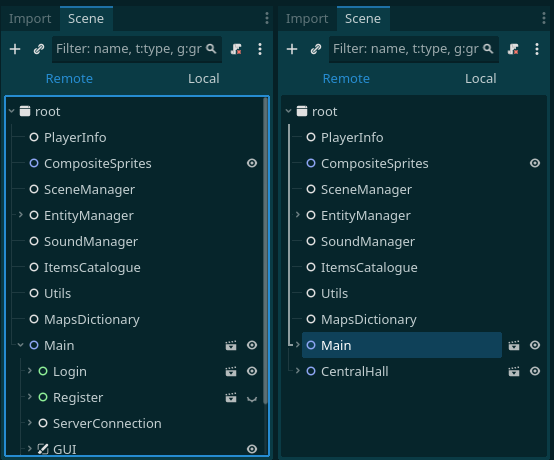
\includegraphics[width=0.6\textwidth]{../assets/godot-scene-tree.png}
    \caption{Izquierda: árbol de nodos (Scene Tree) en la pantalla principal del juego,
             derecha: árbol de nodos cuando el jugador está en un nivel del juego.}
    \label{fig:godot-node-tree}
\end{figure}


Cuando un jugador ejecuta por primera vez el juego, lo primero que verá es la escena del menú principal.
Luego de elegir el idioma del juego, tendrá dos opciones disponibles: ingresar al juego
con un usuario existente desde el Login o crear un personaje y un usuario en CharacterCreation (también
llamada Register).

\begin{figure}[htbp]
    \centering
    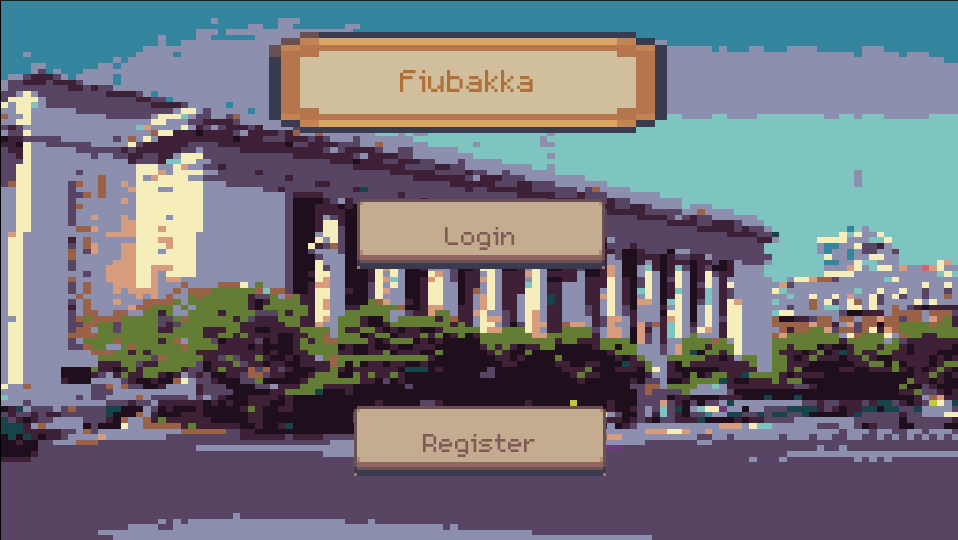
\includegraphics[width=0.7\textwidth]{../assets/godot-main-menu.png}
    \caption{Pantalla del Menú Principal}
    \label{fig:godot-main-menu}
\end{figure}

\newpage

Si el usuario opta por ingresar al juego a través de Login, deberá ingresar con un nombre de usuario
y contraseña existentes. En caso de haber algún error de login, se mostrará por pantalla el error 
correspondiente, como por ejemplo credenciales inválidas. Como el sistema de autenticación de usuario no
fue el foco de este proyecto, no es posible recuperar la contraseña de un usuario ni tampoco eliminarlo.

\begin{figure}[htbp]
    \centering
    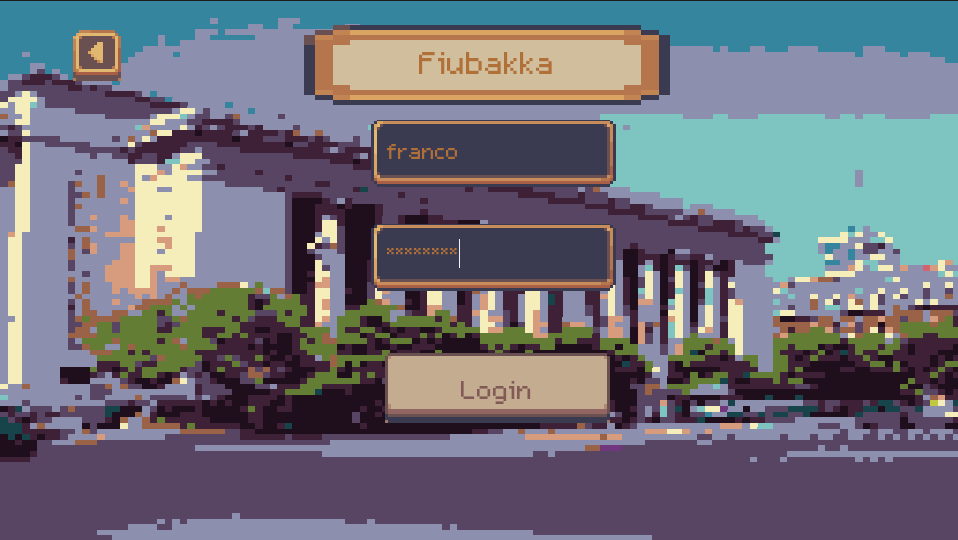
\includegraphics[width=0.7\textwidth]{../assets/godot-login.png}
    \caption{Pantalla de Login. Son necesarios un nombre de usuario y contraseña.}
    \label{fig:godot-login}
\end{figure}

Por otro lado, si se tratase de un nuevo jugador o si se desea crear otro personaje, el usuario
puede entrar a la pantalla de registro donde podrá ingresar sus nuevas
credenciales de usuario y también personalizar la apariencia de su nuevo personaje. En esta pantalla
se visualiza del lado izquierdo un \textit{sprite} del personaje que será creado y a la derecha una
lista de selectores para los distintos cosméticos que componen al \textit{sprite}. El usuario podrá
agregar, combinar e incluso quitar los cosméticos de su personaje a su gusto. Una vez que haya hecho su elección
e ingrese sus credenciales, se crea el usuario correspondiente.

\begin{figure}[htbp]
    \centering
    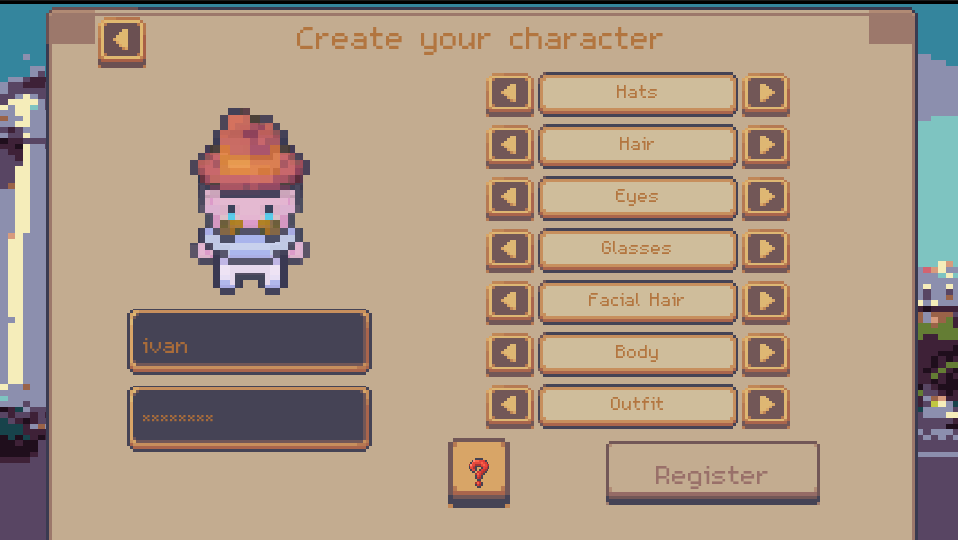
\includegraphics[width=1.0\textwidth]{../assets/godot-register.png}
    \caption{Pantalla de creación de personaje.}
    \label{fig:godot-register}
\end{figure}

Un feature del cual hacemos uso en Godot es el de los scripts \textbf{Autoloads}, que funcionan de manera
similar a las clases \textbf{Singleton} del patrón de diseño del mismo nombre.
Estos Autoloads se cargan en el arbol de escenas desde el comienzo y están siempre disponibles
sin importar cual es la escena actualmente activa. Un detalle importante es que
estos Autoloads no son Singletons propiamente dichos, sino que simplemente actúan como tales. Esto quiere
decir que se podría crear más de una instancia de un script Autoload. Sin embargo, este no fue el caso
para los Autoloads que desarrollamos.
Se definieron ciertas clases que son necesarias en un scope global como Autoloads.
Por ejemplo, para el manejo, carga y borrado de escenas, hacemos uso de un \textbf{SceneManager}, 
que es un script Autoload que permite transicionar entre niveles dentro del juego. En general, 
se implementaron Singletons de estilo \textit{Manager} para acceder a distintos comportamientos y 
configuraciones globales (información del jugador, cambio de escenas, control de entidades, entre otros).

Cada nivel es una instancia de la clase \textbf{Level}, la cual define el comportamiento común
necesario, principalmente el manejo de las puertas y transición entre niveles.
Si bien cada escena de nivel fue diseñada de forma especial para replicar alguna parte de la arquitectura de la Facultad de Ingeniería,
existen ciertos tipos de nodos que deben usarse en todos los niveles (ver Figura \ref{fig:level-nodes}).
Por ejemplo, para definir la forma, apariencia y estructura de cada nivel, debe tener un \textbf{TileMap} asociado.
Se trata de un nodo que a partir de una textura permite "pintar" sobre
una grilla predefinida de pixeles, como si fuera un canvas. Además se deben definir las colisiones de las 
paredes de cada nivel, para que el jugador no se pase del límite de la cámara ni se vaya 
\textit{out of bounds}. Esto se logra con nodos del tipo \textbf{StaticBody2D} y \textbf{CollisionShape2D},
definiendo su posición y la forma de la colisión.
Otro nodo importante en un nivel es el \textbf{Player}, ya que cada nivel debe incluir su propio jugador.
Esto quiere decir que no existe un Player único que transferimos entre los distintos 
niveles, sino que cada instancia de Level debe recrear al nodo Player. Esta implementación
simplifica la transferencia de data necesaria entre niveles.
También son importantes las puertas o \textbf{Doors} en los niveles, ya que estas cumplen la función de
permitirles a los jugadores cambiar de nivel y moverse a través de la Facultad.

\begin{figure}[htbp]
    \centering
    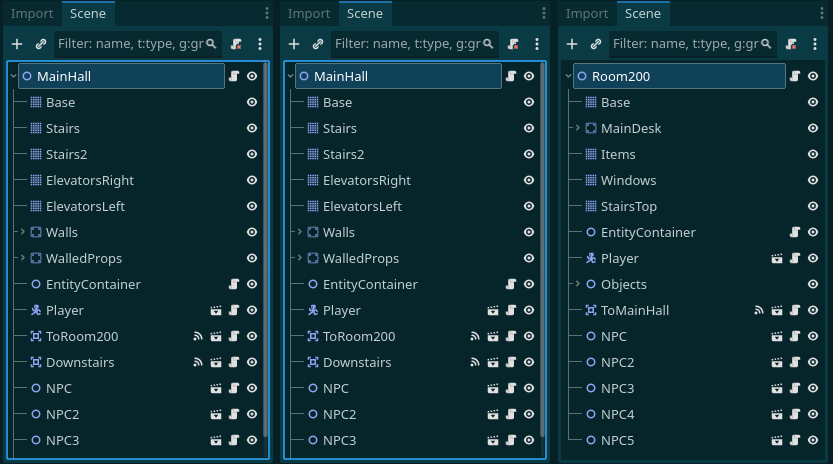
\includegraphics[width=1.0\textwidth]{../assets/levels-tree-nodes.png}
    \caption{Ejemplos de árboles de nodos para distintas escenas de tipo \textit{Level}. Nótese que
            comparten ciertos tipos de nodos en común (Player, TileMaps, CollisionShape2D, etc.)}
    \label{fig:level-nodes}
\end{figure}

Como se mencionó anteriormente, para transicionar entre niveles, es decir, para cargar un nuevo Level
y remover el actual, implementamos un script Autoload llamado \textbf{SceneManager}.
Este SceneManager encapsula la responsabilidad de manejar el cambio de niveles de forma natural para 
el usuario. El proceso para cambiar de un nivel a otro es:

\begin{itemize}
    \item Mostrar una escena de pantalla de carga \textbf{LoadingScreen} (Figura \ref{fig:loading-screen}).
    \item Esperar la respuesta del servidor con la confirmación de la transición al nuevo mapa.
    \item Cargar en memoria la nueva escena en un hilo separado.
    \item Una vez cargada la escena nueva, montarla en el arbol de escenas.
    \item Antes de remover la escena actual, transferir cualquier tipo de data relevante de un nivel a otro,
    como por ejemplo el equipamiento del jugador.
    \item Remover la escena actual.
    \item Remover la LoadingScreen.
\end{itemize}

\begin{figure}[htbp]
    \centering
    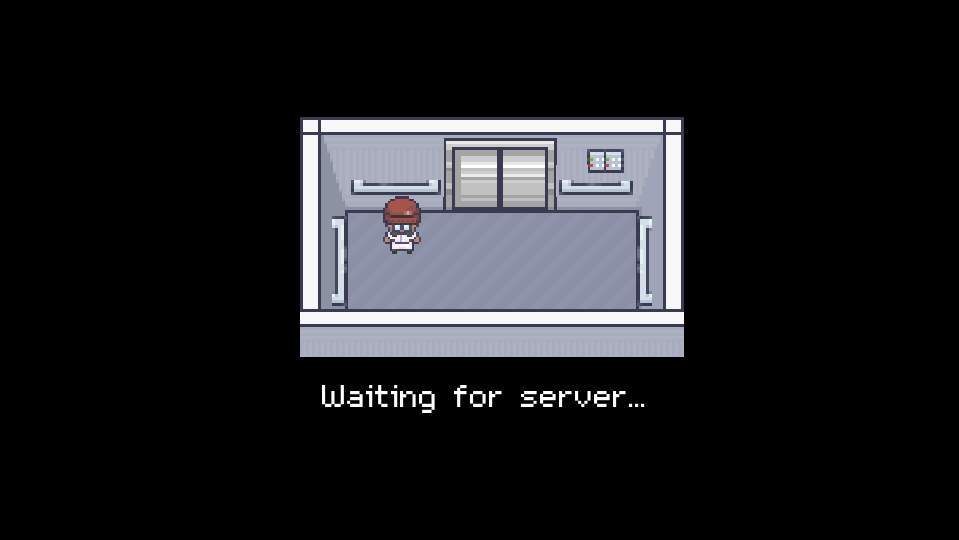
\includegraphics[width=1.0\textwidth]{../assets/godot-loading-screen.png}
    \caption{Pantalla de carga.}
    \label{fig:loading-screen}
\end{figure}

Un Player o jugador es una escena donde se encapsulan tanto la vista como el comportamiento del
personaje que controla el usuario. Está compuesto tanto de \textbf{CompositeSprites} para la visualización
de los cosméticos elegidos en la pantalla de creación del personaje o mediante los ítems de su inventario, como de CollisionShape2D para
la detección de colisiones con las paredes u otros objetos del nivel donde se encuentre.
Además es esta escena la que contiene una \textbf{Camera2D}, que representa la vista que el usuario tendrá
del juego en el \textit{viewport} de su pantalla. Al ser un subnodo del Player, logramos un efecto donde la
cámara sigue al jugador a donde sea que vaya, como es usual en este tipo de juegos. Cabe destacar que se 
definieron coordenadas límites para la cámara (o \textit{bounds}) para evitar que se muestren regiones por
fuera del perímetro de cada mapa.
Otro nodo notable es el AnimationPlayer, el cual permite definir animaciones para el jugador
(por ejemplo, \textit{idle} o \textit{walking}) definiendo cuál \textit{sprite} debe mostrarse en cada
\textit{frame} de la animación.

Dos escenas muy similares al Player son las \textbf{Entities} y los \textbf{NPCs}.
Ambos cuentan con los mismos nodos que un Player (CompositeSprites, CollisionShape2D, AnimationPlayer),
pero la principal diferencia es que estas escenas no son controladas por el jugador.
Una Entity es el personaje de otro jugador humano conectado. Un NPC (\textit{Non-Playable Character})
es un personaje que no es controlado por una persona. El jugador puede interactuar
con ambos de distintas formas.

Una vez dentro de la Facultad, el jugador podrá moverse a través del nivel usando las cuatro teclas de flechas
direccionales del teclado o \textbf{WASD}.
También podrá acceder a un inventario presionando la tecla \textbf{I} (ver Figura \ref{fig:inventory}).
Dentro de este inventario verá listados los objetos que tenga disponible, ya sean objetos personales u otros
cosméticos. En el caso de los cosméticos, podrá optar por equipar o desesquipárselos, modificando la
apariencia de su personaje.
Además al presionar la tecla \textbf{TAB} abrirá una ventana de chat, donde podrá intercambiar mensajes con
todos los otros jugadores que estén conectados en la misma región de la Facultad (ver Figura \ref{fig:chat}).
Mientras esté chateando, el jugador no podrá moverse y tendrá que cerrar la ventana de chat presionando \textbf{TAB} nuevamente.

\begin{figure}[htbp]
    \centering
    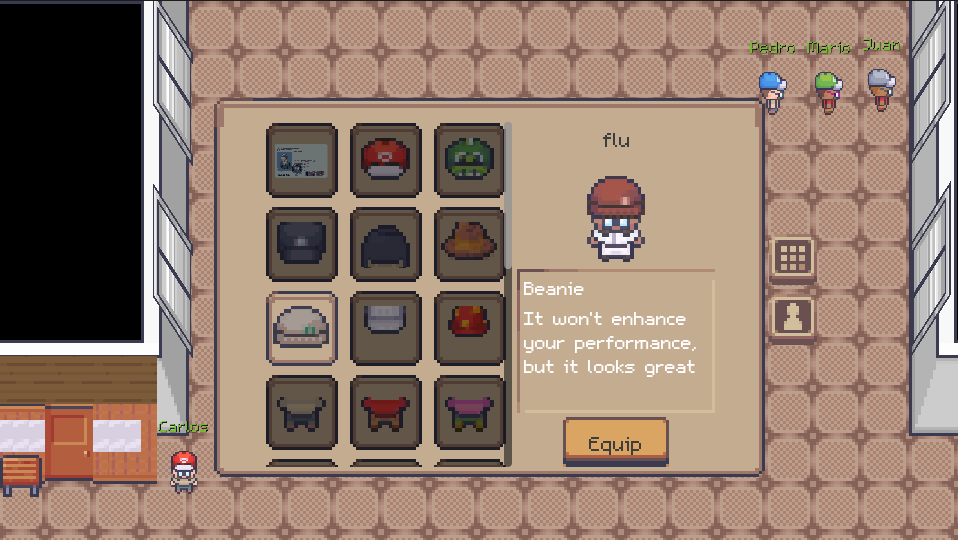
\includegraphics[width=1.0\textwidth]{../assets/godot-inventory.png}
    \caption{Inventario de items.}
    \label{fig:inventory}
\end{figure}

\begin{figure}[htbp]
    \centering
    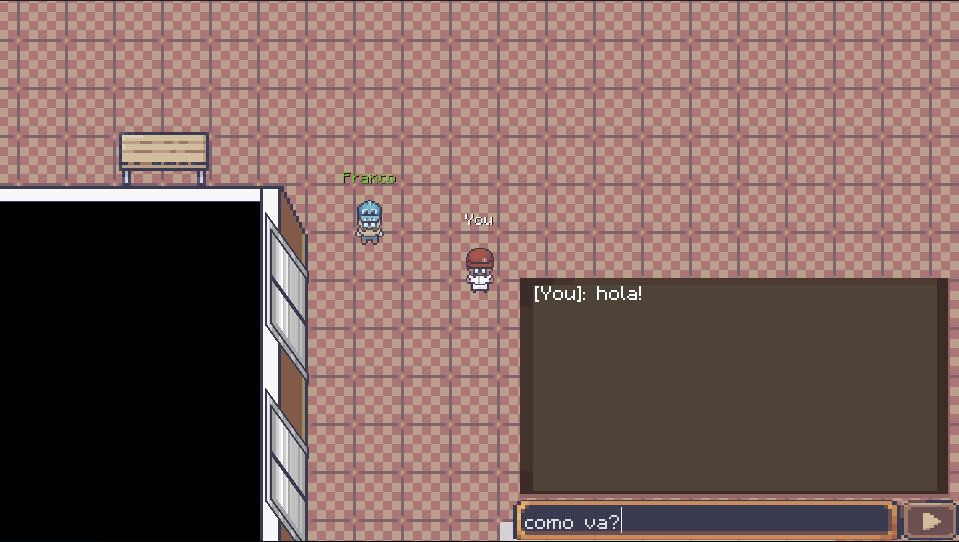
\includegraphics[width=1.0\textwidth]{../assets/godot-chat.png}
    \caption{Chat.}
    \label{fig:chat}
\end{figure}

Uno de los principales features del juego es la posibilidad de desafiar a otros jugadores a una partida de 
Truco. El Truco es un juego de cartas argentino que se juega con naipes españoles. El objetivo del juego
es obtener 30 puntos antes que el oponente, ganando las manos y haciendo distintas jugadas con cantos.
Para desafiar a otro jugador a una partida de Truco, el usuario solo debe hacer click derecho sobre cualquier
otro personaje (no NPC) que vea en su pantalla. Eso habilitará un submenú con un botón para jugar al Truco.
El otro jugador recibirá una notificación que puede aceptar o rechazar. Al aceptarla, ambos jugadores
verán la pantalla de Truco y la partida comienza. (Figuras \ref{fig:truco-submenu} y \ref{fig:truco-notification})

\begin{figure}[htbp]
    \centering
    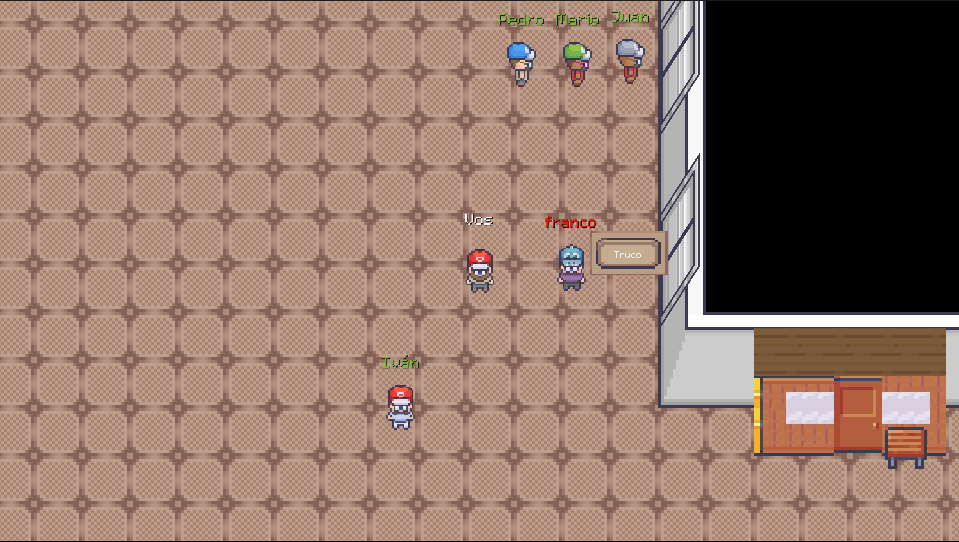
\includegraphics[width=1.0\textwidth]{../assets/godot-truco-menu.png}
    \caption{Submenú de jugador. A partir de este menú se puede desafiar a otro jugador al Truco.}
    \label{fig:truco-submenu}
\end{figure}

\begin{figure}[htbp]
    \centering
    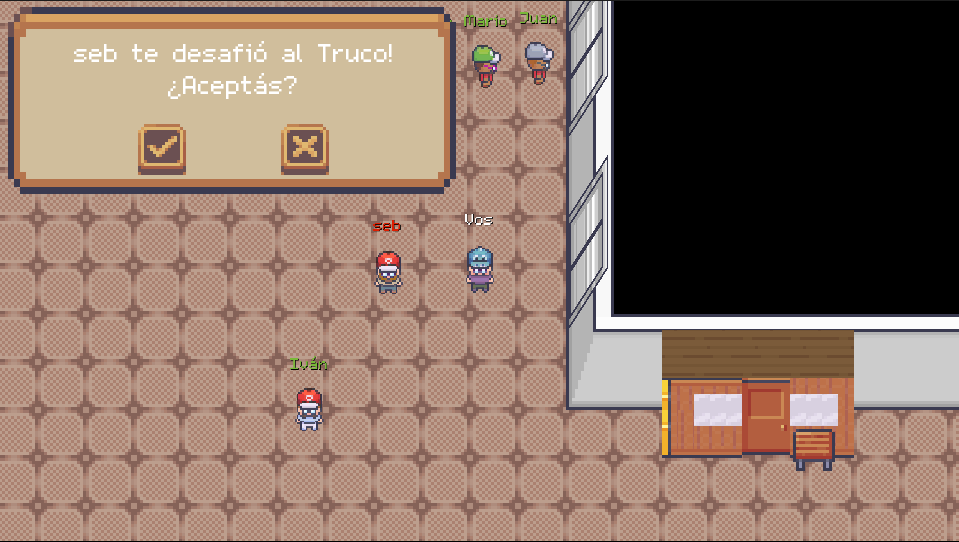
\includegraphics[width=1.0\textwidth]{../assets/godot-truco-notification.png}
    \caption{Notificación de Truco. El jugador puede rechazarla o aceptarla y empezar la partida inmediatamente.}
    \label{fig:truco-notification}
\end{figure}

Los jugadores verán las cartas de su mano en la región inferior de la pantalla, así como también las opciones
de cantos disponibles en dicho turno, como se muestra en la Figura \ref{fig:truco-game}.
Para hacer un canto, solo deben hacer click en el botón correspondiente
y esperar la respuesta del oponente. Para jugar un carta, el jugador que corresponda podrá arrastrarla con el
mouse desde su mano y soltarla sobre la mesa en la región que corresponda al turno que está transcurriendo,
lo que se conoce como \textit{drag and drop}. El otro jugador va a ver la carta jugada por su oponente y se le habilitará
su turno si es que aún no terminó la ronda.
La partida termina cuando un jugador llega a acumular 30 puntos o en caso de que alguno abandone, ya sea 
voluntariamente o por alguna desconexión.
Todas las reglas del Truco así como también el control del transcurso de la partida y del \textit{game state}
están implementadas en el servidor. El cliente solo funciona a modo de interfaz para que los
usuarios puedan jugar.

\begin{figure}[htbp]
    \centering
    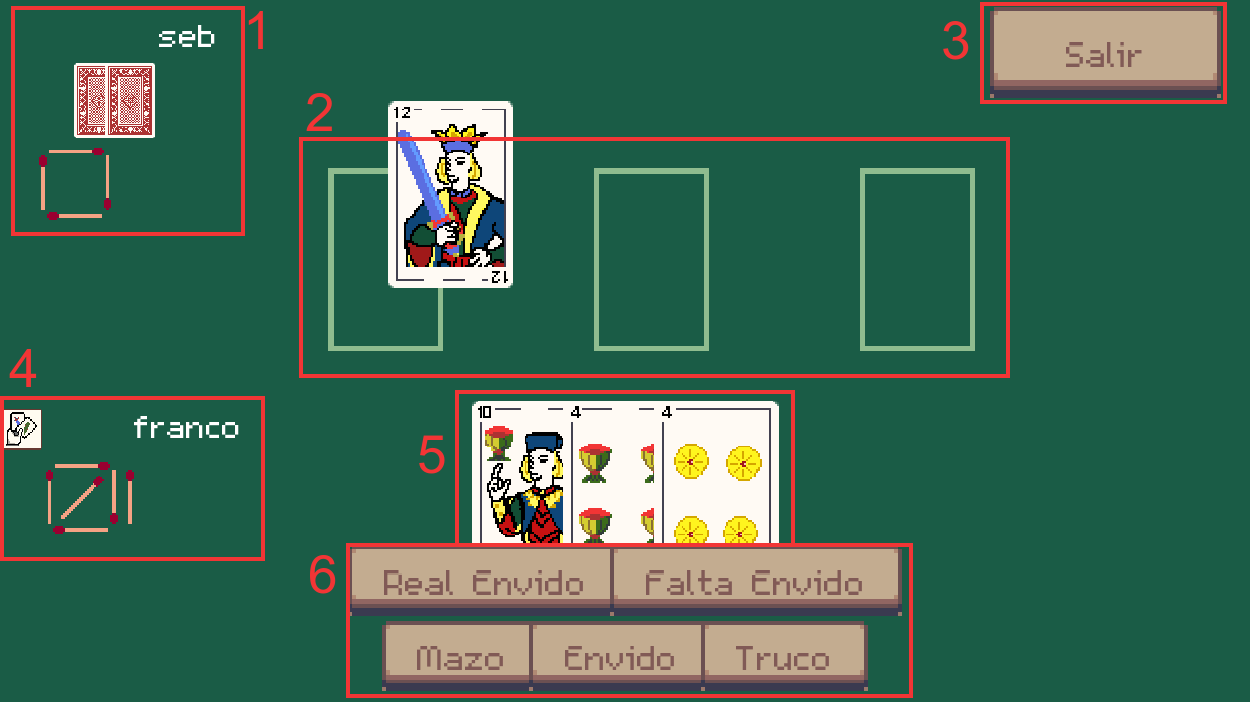
\includegraphics[width=0.8\textwidth]{../assets/godot-truco.png}
    \caption{Pantalla de Truco durante una partida en transcurso. 
             Las regiones numeradas son: región del oponente con nombre, cartas y puntaje (1),
             zona de juego (2), botón para salir (3), región del jugador con nombre, puntaje e
             indicador de turno (4), mano del jugador (5) y cantos disponibles (6).}
    \label{fig:truco-game}
\end{figure}

Todos los controles del juego están detallados en el apéndice \ref{ref:game-controls}.


\subsubsection{Comunicación con el servidor}

\noindent Al comienzo del proyecto, pensamos que un posible limitante de usar Godot podían ser las herramientas
que el motor ofrece para la conectividad con el servidor. 
Afortunadamente, Godot provee APIs para conexiones UDP y TCP que cumplieron con los requisitos
necesarios para implementar nuestro protocolo. En nuestro caso, decidimos usar el protocolo de red TCP debido a los siguientes requisitos
que habíamos establecido para \textit{Fiubakka}:
\begin{itemize}
    \item Conexión persistente con el servidor.
    \item Detección de fallos en la conexión con el servidor.
\end{itemize}

Luego, definimos nuestras propias clases \textit{wrapper} para establecer la conexión al servidor y el 
manejo de mensajes. Para la recepción implementamos un ServerConsumer que se encarga de recibir los paquetes 
del servidor, deserealizar el mensaje (ver sección \ref{sec:events-communication}) y, según el mensaje recibido, 
invocar al \textit{handler} correspondiente para actualizar el estado del juego del lado del cliente.
Este ServerConsumer se ejecuta en un hilo aparte, para no bloquear el hilo principal mientras
esperamos recibir paquetes del servidor. Sin embargo, luego de deseralizar un mensaje recibido, el \textit{handler}
correspondiente se ejecuta en el hilo principal.

El envío de mensajes del cliente hacia el servidor funciona de forma análoga: algún input de un 
usuario dispara una \textit{signal} que el ServerProducer recibe, este se encarga de crear 
el mensaje correspondiente con los parámetros correctos, lo serializa y lo envía al servidor a través de la conexión TCP establecida
al iniciar el juego.

Aún habiendo definido el protocolo de comunicación a utilizar para conectar al cliente y servidor,
fue necesario tomar ciertas decisiones sobre las responsabilidades de cada uno de los dos componentes
y como afectarían al diseño del juego. Esto nos lleva a una característica importante de nuestra arquitectura:
el manejo del movimiento de los jugadores y las colisiones.

\subsubsection{Lógica del juego: movimiento y colisiones}
\label{sec:movement-logic}

\noindent Otro de nuestros problemas iniciales fue decidir cómo implementaríamos el movimiento del 
jugador. Al tratarse de un juego online, lo ideal sería que la lógica fuera mayormente implementada del 
lado del servidor y así garantizar que los jugadores no pudieran realizar movimientos prohibidos, como 
ir a zonas que no estuvieran permitidas u obtener algún tipo de ventaja. Para este caso, Godot únicamente debería comunicar la dirección a la que se desea mover el 
jugador y dejar que el servidor se encargue de verificar que el movimiento es válido, para luego calcular 
la nueva posición del jugador. Por último, el servidor le respondería al cliente de Godot la nueva
posición del jugador para que se vea reflejada en el juego. Esto implicaría que el servidor tendría la responsabilidad
de validar las colisiones.

Sin embargo, se hizo rápidamente aparente
los problemas que esta decisión tendría. Por un lado tendríamos la complejidad de implementar un sistema de colisiones en una arquitectura distribuida,
donde habría que centralizar el estado de las posiciones ocupadas por cada jugador en un único actor, lo cual iría en contra de la distribución de nuestra arquitectura, o implementar
algún sistema de colisiones distribuido, que sería extremadamente complejo y excedería ampliamente el \textit{scope} del proyecto.
Se decidió entonces ceder la mayor parte de la lógica del movimiento al cliente debido a que Godot ya provee 
su propio sistema de colisiones, por lo cual resulta responsabilidad del cliente verificar que el movimiento sea válido y respete las colisiones con los demás
objetos del juego.

Cabe aclarar que esta solución funciona solo para colisiones estáticas, es decir, entre un solo objeto
dinámico (el jugador) y los demás objetos estáticos (el perímetro de un nivel u otros objetos).
Debido a que nuestro juego no tiene colisiones dinámicas (es decir, entre jugadores u objetos móviles) esta restricción
no nos afecta. Es importante sin embargo tenerla en cuenta si se desease desarrollar un videojuego de otras características utilizando
nuestra arquitectura.

\subsection{Juego ejecutable}

\noindent Otro aspecto importante del cliente es poder generar un archivo ejecutable con el juego,
para facilitar el acceso del mismo a los usuarios.
Si bien una forma de poder ejecutarlo es clonando el código fuente y levantando el proyecto vía el editor
de Godot, esta forma no es recomendable por dos razones:

\begin{itemize}
    \item No es muy práctico ni amigable para el usuario no técnico.
    \item Al disponibilizar el código fuente, cualquier usuario podría correr una versión modificada del 
    cliente del juego y conectarse de todas formas al servidor. Existen formas de evitar esto pero no se encuentran
    implementadas en \textit{Fiubakka}.
\end{itemize}

Debido a esto decidimos generar un ejecutable del cliente para poder distribuirlo fácilmente.

Godot provee una forma muy fácil y sencilla de exportar el juego a un ejecutable para distintas plataformas.
Solo es necesario descargar los \textit{templates} correspondientes a la plataforma destino, que pueden ser
distintos sistemas operativos como Windows, Linux o MacOS, así como también otras plataformas, como dispositivos
Android o incluso aplicaciones web.
Para nuestro proyecto generamos ejecutables funcionales para sistemas operativos Windows y Linux.

Como se explicará más adelante, para poder jugar es necesario además conectarse al servidor a través de Cloudflare\ref{ref:cloudflare}.
Es por esto que el jugador deberá instalar el \textit{daemon} de Cloudflare y correr el siguiente comando en una terminal antes de ejecutar el juego:

\begin{lstlisting}[language=bash]
    $ cloudflared access tcp --hostname fiubakka.marcosrolando.uk --url 127.0.0.1:2020
\end{lstlisting}

Para facilitarle el uso al usuario no familiarizado con interfaces de comandos, publicamos además dos
archivos de scripts ejecutables para sistemas Windows y Linux, para la instalación y ejecución de Cloudflared junto con el juego:
\begin{itemize}
    \item \textbf{setup.bat} (Windows) y \textbf{setup.sh} (Linux) para la instalación del \textit{daemon}.
    \item \textbf{play.bat} (Windows) y \textbf{play.sh} (Linux) correr el comando \textit{cloudflared} en simultaneo con el juego.
\end{itemize}
